%!TEX program = xelatex
%!TEX encoding = UTF-8 Unicode
\documentclass[12pt,onlymath]{beamer}
\usefonttheme{serif}


\useinnertheme{rectangles}
\useoutertheme{miniframes}
\usecolortheme{dove}
\setbeamertemplate{navigation symbols}{}
\setbeamercovered{transparent}

% colorbrewer paired colours
\definecolor{lightblue}{RGB}{166,206,227}
\definecolor{darkblue}{RGB}{31,120,180}
\definecolor{lightgreen}{RGB}{178,223,138}
\definecolor{darkgreen}{RGB}{51,160,44}
\definecolor{lightred}{RGB}{251,154,153}
\definecolor{darkred}{RGB}{227,26,28}
\definecolor{lightorange}{RGB}{253,191,111}
\definecolor{darkorange}{RGB}{255,127,0}
\definecolor{lightpurple}{RGB}{202,178,214}
\definecolor{darkpurple}{RGB}{106,61,154}
\definecolor{lightyellow}{RGB}{255,255,153}
\definecolor{darkyellow}{RGB}{177,89,40}

\newcommand{\darkred}[1]{\textcolor{darkred}{{#1}}}
\newcommand{\darkblue}[1]{\textcolor{darkblue}{{#1}}}
\newcommand{\darkorange}[1]{\textcolor{darkorange}{{#1}}}
\newcommand{\darkgreen}[1]{\textcolor{darkgreen}{{#1}}}
\newcommand{\darkpurple}[1]{\textcolor{darkpurple}{{#1}}}
\newcommand{\darkyellow}[1]{\textcolor{darkyellow}{{#1}}}

% base16 solarized colours
\definecolor{b16Black}{HTML}{2D2D2D} % # Base 00 - Black
\definecolor{b16Red}{HTML}{F2777A} % # Base 08 - Red
\definecolor{b16Green}{HTML}{99CC99} % # Base 0B - Green
\definecolor{b16Yellow}{HTML}{FFCC66} % # Base 0A - Yellow
\definecolor{b16Blue}{HTML}{6699CC} % # Base 0D - Blue
\definecolor{b16Magenta}{HTML}{CC99CC} % # Base 0E - Magenta
\definecolor{b16Cyan}{HTML}{66CCCC} % # Base 0C - Cyan
\definecolor{b16White}{HTML}{D3D0C8} % # Base 05 - White
\definecolor{b16BrightBlack}{HTML}{747369} % # Base 03 - Bright Black
\definecolor{b16BrightWhite}{HTML}{F2F0EC} % # Base 07 - Bright White

% base16 eighties colours
\definecolor{b1600}{HTML}{2D2D2D}
\definecolor{b1601}{HTML}{393939}
\definecolor{b1602}{HTML}{515151}
\definecolor{b1603}{HTML}{747369}
\definecolor{b1604}{HTML}{A09F93}
\definecolor{b1605}{HTML}{D3D0C8}
\definecolor{b1606}{HTML}{E8E6DF}
\definecolor{b1607}{HTML}{F2F0EC}
\definecolor{b1608}{HTML}{F2777A}
\definecolor{b1609}{HTML}{F99157}
\definecolor{b160A}{HTML}{FFCC66}
\definecolor{b160B}{HTML}{99CC99}
\definecolor{b160C}{HTML}{66CCCC}
\definecolor{b160D}{HTML}{6699CC}
\definecolor{b160E}{HTML}{CC99CC}
\definecolor{b160F}{HTML}{D27B53}

\newcommand{\red}[1]{\textcolor{b1608}{{#1}}}
\newcommand{\blue}[1]{\textcolor{b160D}{{#1}}}
\newcommand{\orange}[1]{\textcolor{b1609}{{#1}}}
\newcommand{\green}[1]{\textcolor{b160B}{{#1}}}
\newcommand{\purple}[1]{\textcolor{b160E}{{#1}}}
\newcommand{\brown}[1]{\textcolor{b160F}{{#1}}}
\newcommand{\cyan}[1]{\textcolor{b160C}{{#1}}}
\newcommand{\yellow}[1]{\textcolor{b160A}{{#1}}}


\setbeamertemplate{frametitle}
{
    \nointerlineskip
    \begin{beamercolorbox}[sep=0.3cm,wd=\paperwidth]{frametitle}
        \vbox{}\vskip-2ex%
        \strut\insertframetitle\strut
        \vskip-0.8ex%
    \end{beamercolorbox}
}
\setbeamercolor{palette quaternary}{fg=b1606,bg=b1601}
\setbeamercolor{titlelike}{parent=palette quaternary}



% xetex specific stuff
\usepackage{xunicode} % unicode support for xetex
\usepackage{fontspec} % font selection for xetex
\DeclareTextCommandDefault{\nobreakspace}{\leavevmode\nobreak\ } 

% set the font
\defaultfontfeatures{Mapping=tex-text}
\setromanfont[Scale=1]{Times}
\setsansfont[Scale=1]{Gill Sans}

\ProvidesPackage{preamble}

\usepackage{url}
\usepackage{array}
\usepackage{amsmath,amssymb,amsfonts,textcomp,amsthm}
\usepackage{booktabs}
\usepackage{relsize}
\usepackage{nicefrac}
\usepackage{graphicx}
\usepackage{rotating}
\usepackage{nth}
\usepackage{acronym}
\usepackage{bm}
%\usepackage{caption} \DeclareCaptionType{copyrightbox}
\usepackage{footnote}
\usepackage{color}

\usepackage{tabularx}
\newcolumntype{x}[1]{>{\centering\arraybackslash\hspace{0pt}}m{#1}}
\newcommand{\tabbox}[1]{#1}

\usepackage{hyperref}
\definecolor{mydarkblue}{rgb}{0,0.08,0.45}
\hypersetup{
    pdftitle={},
    pdfauthor={},
    pdfsubject={},
    pdfkeywords={},
    pdfborder=0 0 0,
    pdfpagemode=UseNone,
    colorlinks=true,
    linkcolor=mydarkblue,
    citecolor=mydarkblue,
    filecolor=mydarkblue,
    urlcolor=mydarkblue,
    pdfview=FitH}

\newcommand{\asdf}{$^{\textnormal{th}}$}

\newcommand{\binarysum}{\sum_{\bf{x} \in \{0,1\}^D}}
\newcommand{\expect}{\mathbb{E}}
\newcommand{\expectargs}[2]{\mathbb{E}_{#1} \left[ {#2} \right]}
\newcommand{\var}{\mathbb{V}}
\newcommand{\varianceargs}[2]{\mathbb{V}_{#1} \left[ {#2} \right]}
\newcommand{\variance}{\mathbb{V}}
\newcommand{\cov}{\operatorname{cov}}
\newcommand{\Cov}{\operatorname{Cov}}
\newcommand{\covarianceargs}[2]{\Cov_{#1} \left[ {#2} \right]}
\newcommand{\colvec}[2]{\left[ \begin{array}{c} {#1} \\ {#2} \end{array} \right]}
\newcommand{\tbtmat}[4]{\left[ \begin{array}{cc} {#1} & {#2} \\ {#3} & {#4} \end{array} \right]}

%\newcommand{\covskinny}[2]{\var\!\left(#1\middle\vert#2\right)} 

\newcommand{\acro}[1]{\textsc{#1}}
%\newcommand{\vect}[1]{\boldsymbol{#1}}
\newcommand{\vect}[1]{{\bf{#1}}}
\newcommand{\mat}[1]{\mathbf{#1}}
\newcommand{\pderiv}[2]{\frac{\partial #1}{\partial #2}}
\newcommand{\npderiv}[2]{\nicefrac{\partial #1}{\partial #2}}

\newcommand{\pha}{^{\phantom{:}}}

\newcommand{\argmin}{\operatornamewithlimits{argmin}}
\newcommand{\argmax}{\operatornamewithlimits{argmax}}

% The following designed for probabilities with long arguments

\newcommand{\Prob}[2]{P\!\left(\,#1\;\middle\vert\;#2\,\right)}
\newcommand{\ProbF}[3]{P\!\left(\,#1\!=\!#2\;\middle\vert\;#3\,\right)}
\newcommand{\p}[2]{p\!\left(#1\middle\vert#2\right)}
\newcommand{\po}[1]{p\!\left(#1\right)}
\newcommand{\pF}[3]{p\!\left(\,#1\!=\!#2\;\middle\vert\;#3\,\right)} 
\newcommand{\mean}[2]{{m}\!\left(#1\middle\vert#2\right)}
%\newcommand{\novmean}[2]{{m}\!\left(#1\middle\vert#2\right)}
%\newcommand{\novcov}[2]{\var\!\left(#1\middle\vert#2\right)}
%\newcommand{\cov}[2]{\var\!\left(#1\middle\vert#2\right)} 
%\newcommand{\pskinny}[2]{p\!\left(#1\;\middle\vert\;#2\right)}
%\newcommand{\meanskinny}[2]{{m}\!\left(#1\middle\vert#2\right)}
%\newcommand{\covskinny}[2]{\var\!\left(#1\middle\vert#2\right)} 

\newcommand{\vI}{\mat{I}}
\newcommand{\vX}{\mat{X}}
\newcommand{\vY}{\mat{Y}}
\newcommand{\vZ}{\mat{Z}}
\newcommand{\vK}{\mat{K}}
\newcommand{\vs}{\vect{s}}
\newcommand{\va}{\vect{a}}
\newcommand{\vA}{\vect{A}}
\newcommand{\vb}{\vect{b}}
\newcommand{\vB}{\mat{B}}
\newcommand{\vR}{\mat{R}}
\newcommand{\vS}{\mat{S}}
\newcommand{\vu}{\vect{u}}
\newcommand{\vk}{\vect{k}}
\newcommand{\vc}{\vect{c}}
\newcommand{\vC}{\mat{C}}
\newcommand{\vw}{\vect{w}}
\newcommand{\vx}{\vect{x}}
\newcommand{\vy}{\vect{y}}
\newcommand{\vz}{\vect{z}}
\newcommand{\vmu}{\vect{\mu}}
\newcommand{\vpi}{\vect{\pi}}
\newcommand{\vphi}{\vect{\phi}}
\newcommand{\vSigma}{\mat{\Sigma}}
\newcommand{\vtheta}{\vect{\theta}}
\newcommand{\vl}{\vect{l}}
\newcommand{\vq}{\vect{q}}
\newcommand{\vf}{\vect{f}}
\newcommand{\vg}{\vect{g}}
\newcommand{\vell}{\vect{\ell}}
\newcommand{\ve}{\vect{\epsilon}}
\newcommand{\vzero}{\vect{0}}
\newcommand{\vone}{\vect{1}}

\newcommand{\He}{\mathcal{H}}
\newcommand{\normx}[2]{\left\|#1\right\|_{#2}}
\newcommand{\Hnorm}[1]{\normx{#1}{\He}}
\newcommand{\mmd}{{\rm MMD}}


\newcommand{\mf}{\bar{\vf}}

\newcommand{\st}{_\star}

\newcommand{\inv}{^{{\mathsmaller{-1}}}}
\newcommand{\tohalf}{^{{\mathsmaller{\nicefrac{1}{2}}}}}

\newcommand{\Normal}{\mathcal{N}}
\newcommand{\N}[3]{\mathcal{N}\!\left(#1|#2,#3\right)}
\newcommand{\Nt}[2]{\mathcal{N}\!\left(#1,#2\right)}
\newcommand{\bN}[3]{\mathcal{N}\big(#1|#2,#3\big)}
\newcommand{\boldN}[3]{\text{\textbf{\mathcal{N}}}\big(#1;#2,#3\big)}
\newcommand{\ones}[1]{\mat{1}_{#1}}
\newcommand{\eye}[1]{\mat{E}_{#1}}
\newcommand{\tra}{{^\ensuremath{\mathsf{T}}}}
\newcommand{\trace}{\operatorname{tr}}
\newcommand{\deq}{:=}
\newcommand{\degree}{^\circ}

\newcommand{\GPt}[2]{\mathcal{GP}\!\left(#1,#2\right)}

\DeclareMathOperator{\chol}{chol}
\DeclareMathOperator{\diag}{diag}

\newcommand{\gp}{{\acro{gp}}}
\newcommand{\gplvm}{{\acro{gp-lvm}}}
\newcommand{\bmc}{{\acro{bmc}}}
\newcommand{\bq}{{\acro{bq}}}
\newcommand{\sbq}{{\acro{sbq}}}

\newenvironment{narrow}[2]{%
  \begin{list}{}{%
  \setlength{\topsep}{0pt}%
  \setlength{\leftmargin}{#1}%
  \setlength{\rightmargin}{#2}%
  \setlength{\listparindent}{\parindent}%
  \setlength{\itemindent}{\parindent}%
  \setlength{\parsep}{\parskip}}%
\item[]}{\end{list}}



\newcommand{\dist}{\ \sim\ }
\def\given{\,|\,}

% Table stuff
\newcolumntype{C}[1]{>{\centering\let\newline\\\arraybackslash\hspace{0pt}}m{#1}}
\newcolumntype{L}[1]{>{\raggedright\let\newline\\\arraybackslash\hspace{0pt}}m{#1}}
\newcolumntype{R}[1]{>{\raggedleft\let\newline\\\arraybackslash\hspace{0pt}}m{#1}}


\def\ie{i.e.\ }
\def\eg{e.g.\ }
\def\iid{i.i.d.\ }
%\def\simiid{\sim_{\mbox{\tiny iid}}}
\def\simiid{\overset{\mbox{\tiny iid}}{\sim}}
\def\eqdist{\stackrel{\mbox{\tiny d}}{=}}
\newcommand{\distas}[1]{\mathbin{\overset{#1}{\kern\z@\sim}}}

\def\Reals{\mathbb{R}}

\def\Uniform{\mbox{\rm Uniform}}
\def\Bernoulli{\mbox{\rm Bernoulli}}
\def\GP{\mathcal{GP}}
\def\GPLVM{\mathcal{GP-LVM}}

% Kernel stuff

\def\inputVar{x}
\def\InputVar{X}
\def\InputSpace{\mathcal{X}}
\def\outputVar{y}
\def\OutputSpace{\mathcal{Y}}
\def\function{f}
\def\kernel{k}
\def\KernelMatrix{K}
\def\SumKernel{\sum}
\def\ProductKernel{\prod}
\def\expression{e}

\def\SE{\acro{SE}}
\def\Per{\acro{Per}}
\def\RQ{\acro{RQ}}
\def\Lin{\acro{Lin}}

\def\subexpr{{\cal S}}
\def\baseker{{\cal B}}
\def\numWinners{k}

\newcommand{\kSE}{{\acro{SE}}}
\newcommand{\kPer}{{\acro{Per}}}
\newcommand{\kLin}{{\acro{Lin}}}
\newcommand{\kRQ}{{\acro{RQ}}}


% Proof stuff
\theoremstyle{plain}
\newtheorem{theorem}{Theorem}[section]
\newtheorem{lemma}[theorem]{Lemma}
\newtheorem{prop}[theorem]{Proposition}
\newtheorem*{cor}{Corollary}



\begin{document}

\title{\textbf{\textcolor{b160A}{Raiders of the Lost Architecture:\\Kernels for Bayesian Optimization in Conditional Parameter Spaces}}}

\author{Kevin Swersky, David Duvenaud, Jasper Snoek, Frank Hutter, {\darkorange{Michael A Osborne}}}
% \address{ University of Oxford}

\begin{frame}\frametitle{}
\maketitle
\end{frame}

%%%%%%%%%%%%%%%%%%%%%%%%%%%%%%%%%%%%%%%%%%%%%%%%%%
\begin{frame}

%%%%%%%%%%%%%%%%%%%%%%%%%%%%%%%%%%%%%%%%%%%%%%%%%%
\frametitle{%
	In \purple{Bayesian optimization,} we often search over structures with \cyan{differing numbers of parameters.}
	\\[0.5cm]
	e.g. We may wish to search over \green{neural network} architectures with an \red{unknown number of layers.}
	\\[0.5cm]
	To relate performance data gathered for different architectures, we define \yellow{a new kernel for conditional parameter spaces} that explicitly includes information about which parameters are relevant in a given structure.
}

%%%%%%%%%%%%%%%%%%%%%%%%%%%%%%%%%%%%%%%%%%%%%%%%%%
\end{frame}
%%%%%%%%%%%%%%%%%%%%%%%%%%%%%%%%%%%%%%%%%%%%%%%%%%



%%%%%%%%%%%%%%%%%%%%%%%%%%%%%%%%%%%%%%%%%%%%%%%%%%
\begin{frame}\frametitle{\red{Bayesian optimization} is efficient for expensive and multimodal functions.}
%%%%%%%%%%%%%%%%%%%%%%%%%%%%%%%%%%%%%%%%%%%%%%%%%%
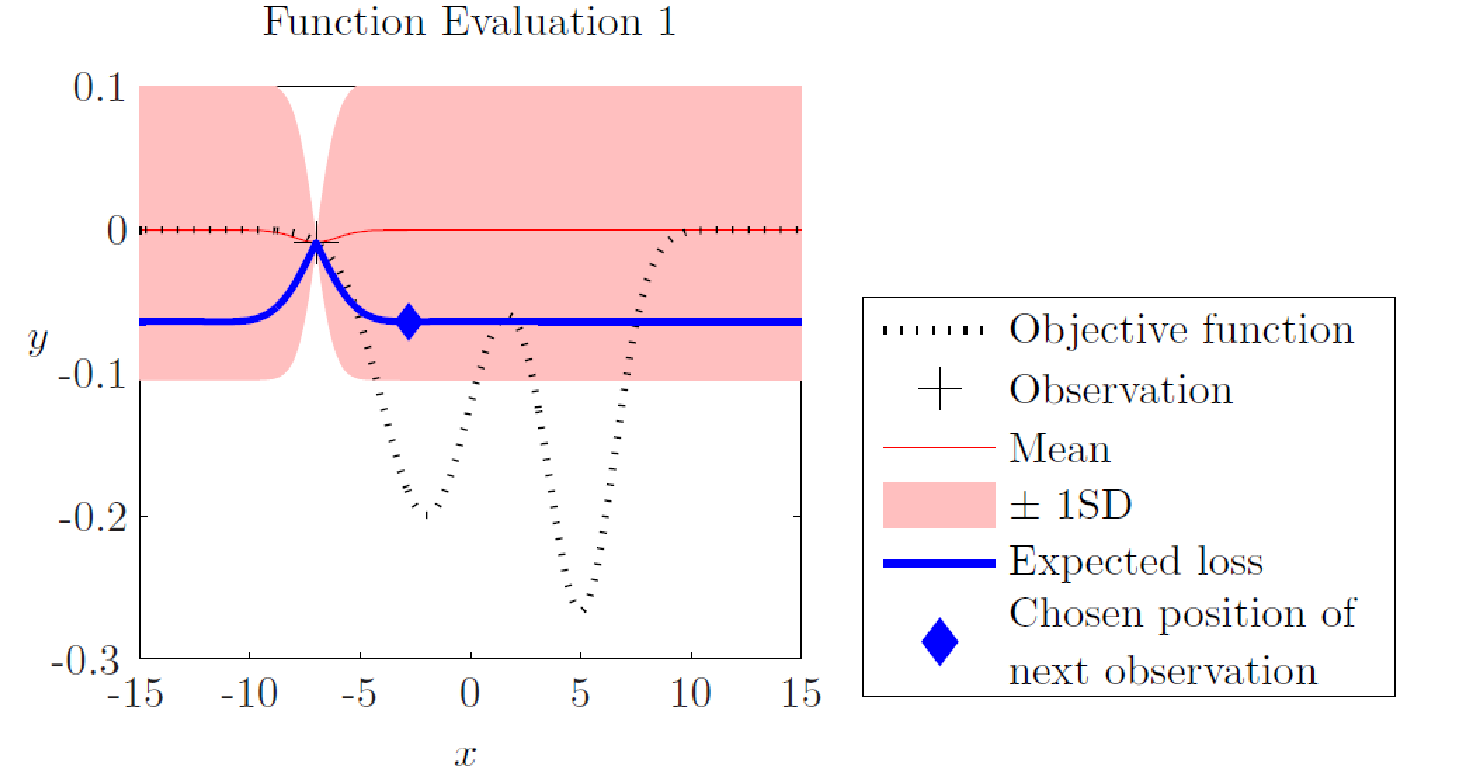
\includegraphics[width = \textwidth]{./figures/bo1.pdf}
%%%%%%%%%%%%%%%%%%%%%%%%%%%%%%%%%%%%%%%%%%%%%%%%%%
\end{frame}
%%%%%%%%%%%%%%%%%%%%%%%%%%%%%%%%%%%%%%%%%%%%%%%%%%
%%%%%%%%%%%%%%%%%%%%%%%%%%%%%%%%%%%%%%%%%%%%%%%%%%
\begin{frame}\frametitle{\red{Bayesian optimization} is efficient for expensive and multimodal functions.}
%%%%%%%%%%%%%%%%%%%%%%%%%%%%%%%%%%%%%%%%%%%%%%%%%%
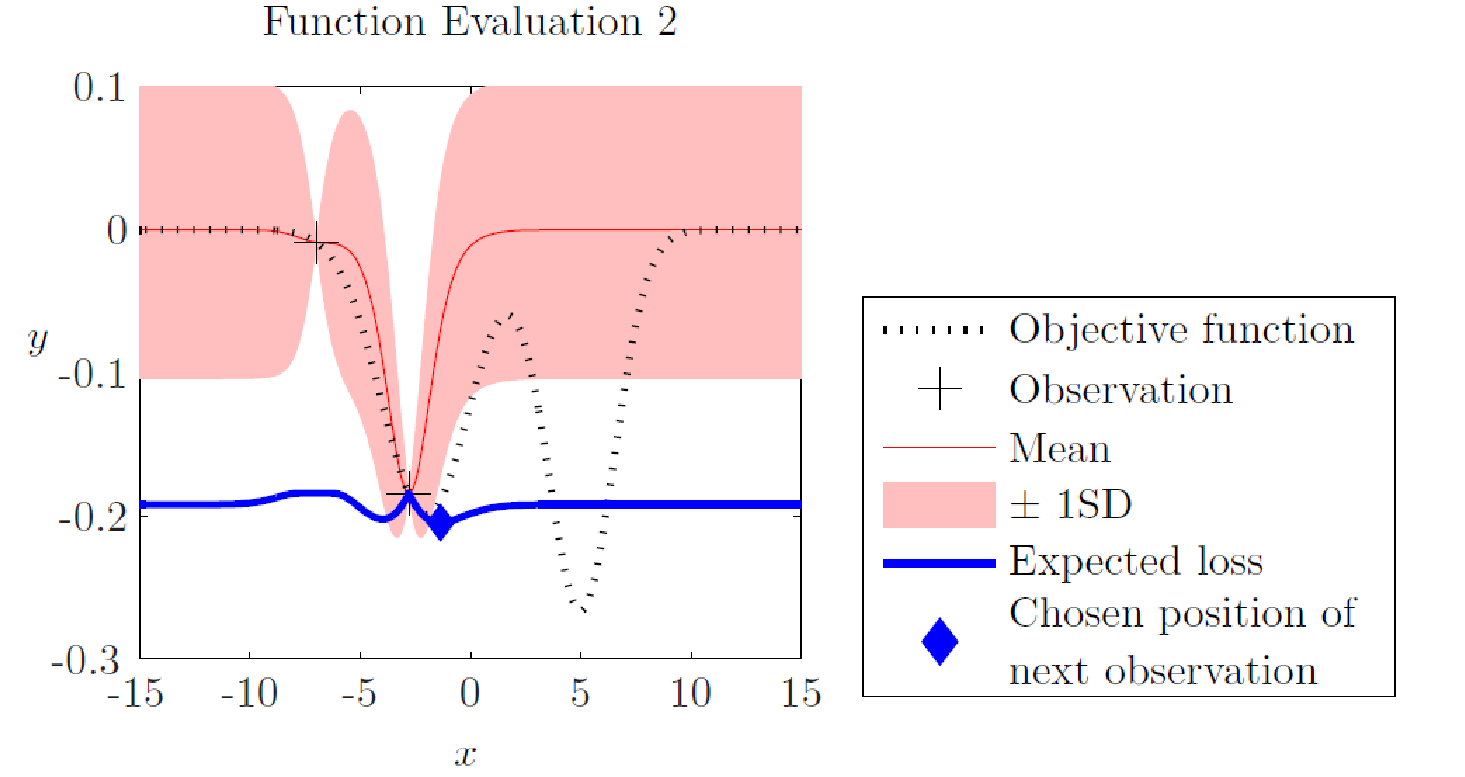
\includegraphics[width = \textwidth]{./figures/bo2.pdf}
%%%%%%%%%%%%%%%%%%%%%%%%%%%%%%%%%%%%%%%%%%%%%%%%%%
\end{frame}
%%%%%%%%%%%%%%%%%%%%%%%%%%%%%%%%%%%%%%%%%%%%%%%%%%
%%%%%%%%%%%%%%%%%%%%%%%%%%%%%%%%%%%%%%%%%%%%%%%%%%
\begin{frame}\frametitle{\red{Bayesian optimization} is efficient for expensive and multimodal functions.}
%%%%%%%%%%%%%%%%%%%%%%%%%%%%%%%%%%%%%%%%%%%%%%%%%%
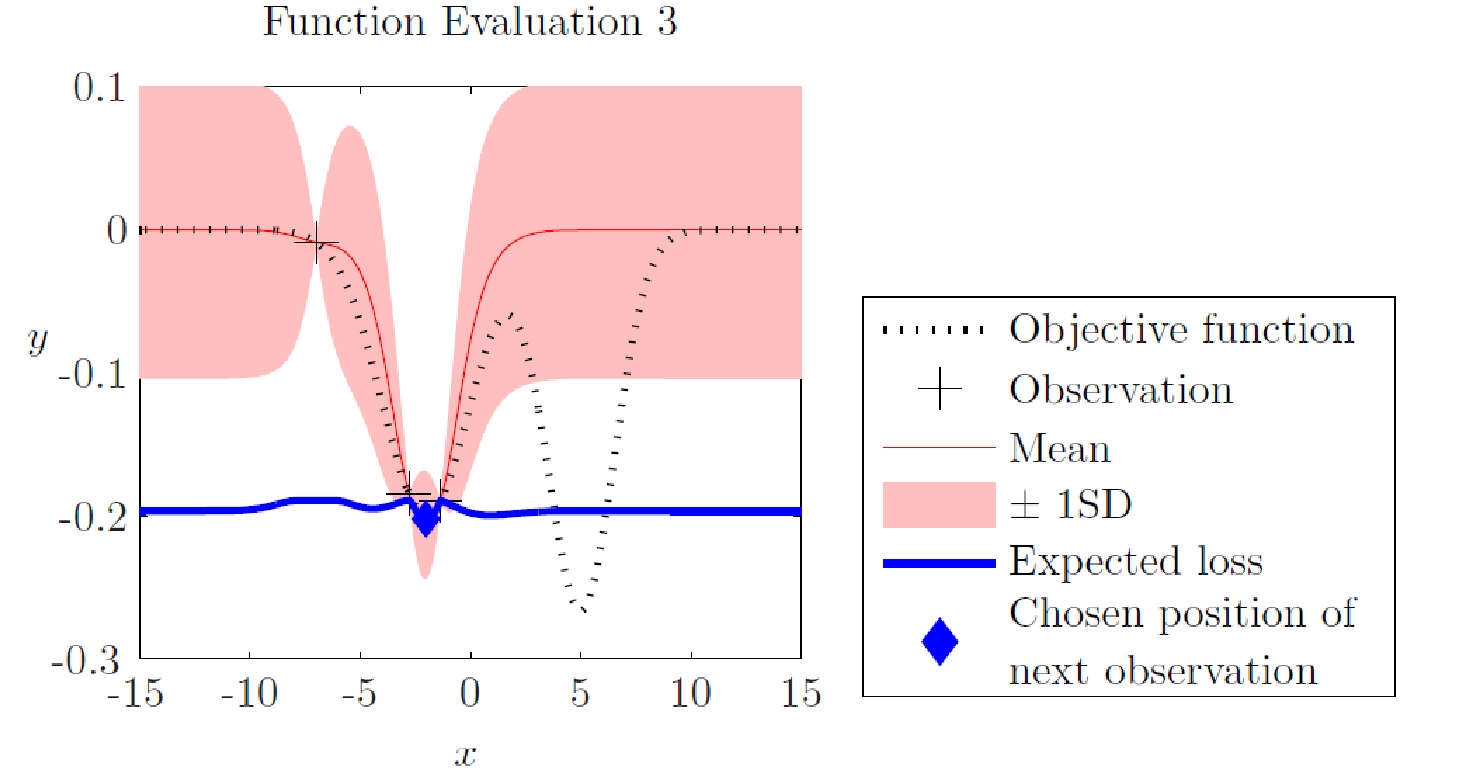
\includegraphics[width = \textwidth]{./figures/bo3.pdf}
%%%%%%%%%%%%%%%%%%%%%%%%%%%%%%%%%%%%%%%%%%%%%%%%%%
\end{frame}
%%%%%%%%%%%%%%%%%%%%%%%%%%%%%%%%%%%%%%%%%%%%%%%%%%
%%%%%%%%%%%%%%%%%%%%%%%%%%%%%%%%%%%%%%%%%%%%%%%%%%
\begin{frame}\frametitle{\red{Bayesian optimization} is efficient for expensive and multimodal functions.}
%%%%%%%%%%%%%%%%%%%%%%%%%%%%%%%%%%%%%%%%%%%%%%%%%%
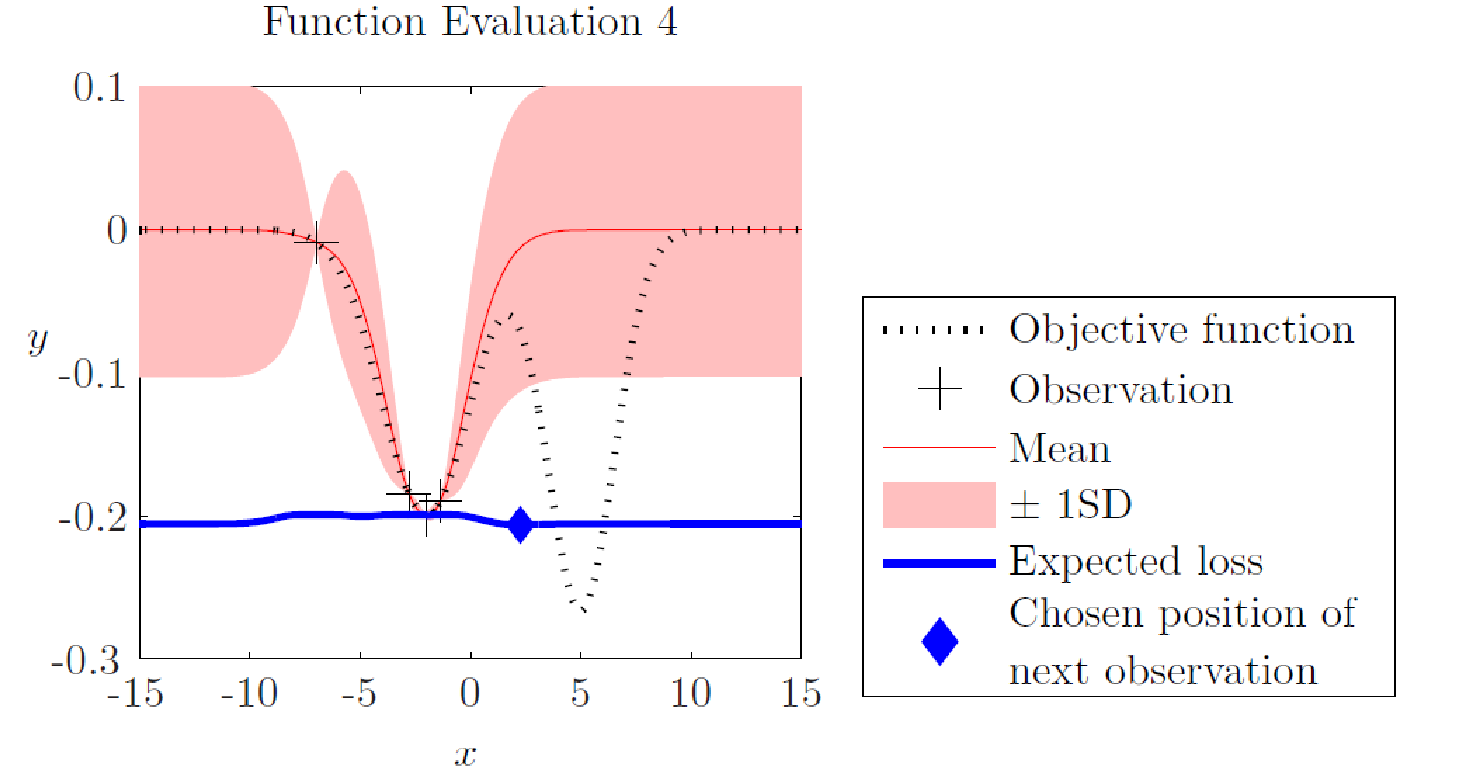
\includegraphics[width = \textwidth]{./figures/bo4.pdf}
%%%%%%%%%%%%%%%%%%%%%%%%%%%%%%%%%%%%%%%%%%%%%%%%%%
\end{frame}
%%%%%%%%%%%%%%%%%%%%%%%%%%%%%%%%%%%%%%%%%%%%%%%%%%
%%%%%%%%%%%%%%%%%%%%%%%%%%%%%%%%%%%%%%%%%%%%%%%%%%
\begin{frame}\frametitle{\red{Bayesian optimization} is efficient for expensive and multimodal functions.}
%%%%%%%%%%%%%%%%%%%%%%%%%%%%%%%%%%%%%%%%%%%%%%%%%%
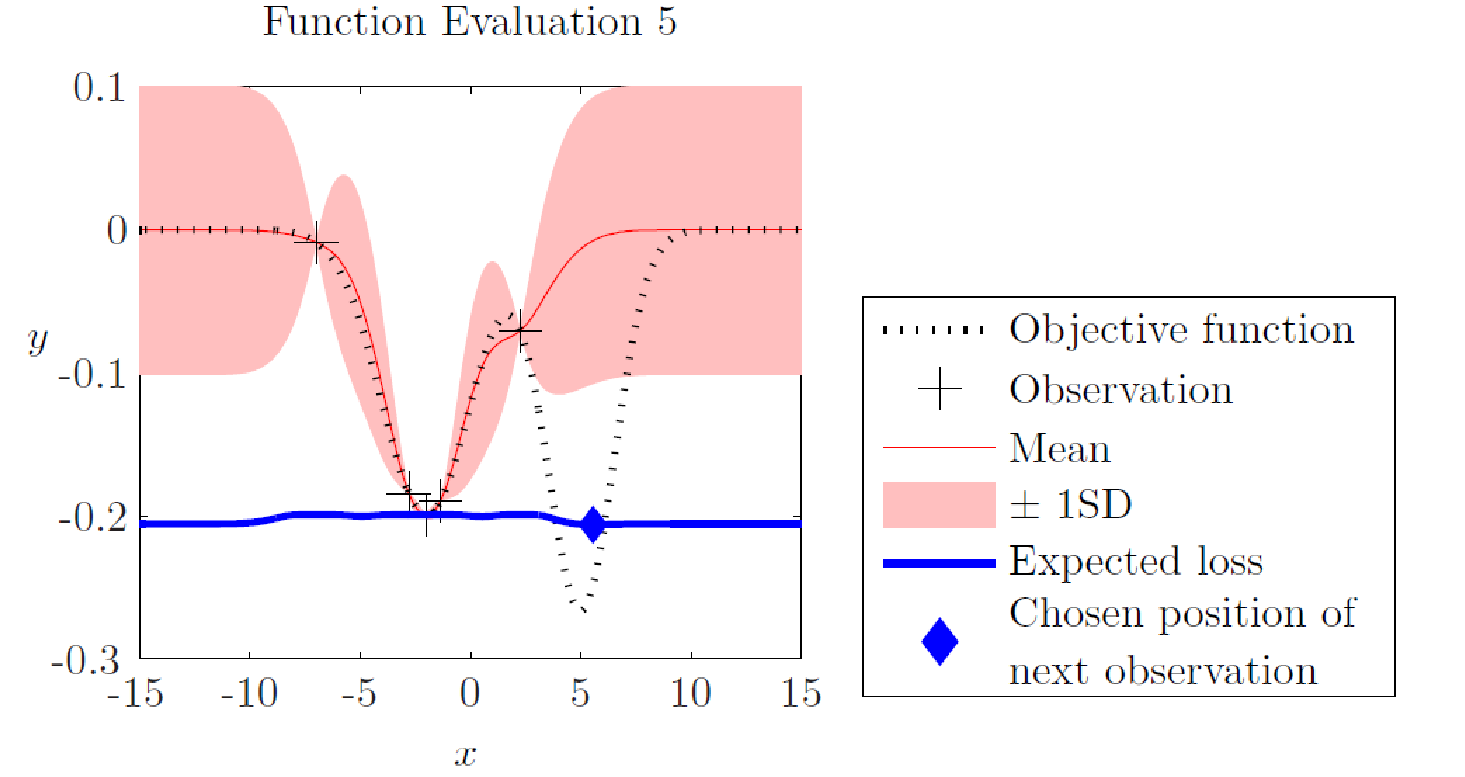
\includegraphics[width = \textwidth]{./figures/bo5.pdf}
%%%%%%%%%%%%%%%%%%%%%%%%%%%%%%%%%%%%%%%%%%%%%%%%%%
\end{frame}
%%%%%%%%%%%%%%%%%%%%%%%%%%%%%%%%%%%%%%%%%%%%%%%%%%
%%%%%%%%%%%%%%%%%%%%%%%%%%%%%%%%%%%%%%%%%%%%%%%%%%
\begin{frame}\frametitle{\red{Bayesian optimization} is efficient for expensive and multimodal functions.}
%%%%%%%%%%%%%%%%%%%%%%%%%%%%%%%%%%%%%%%%%%%%%%%%%%
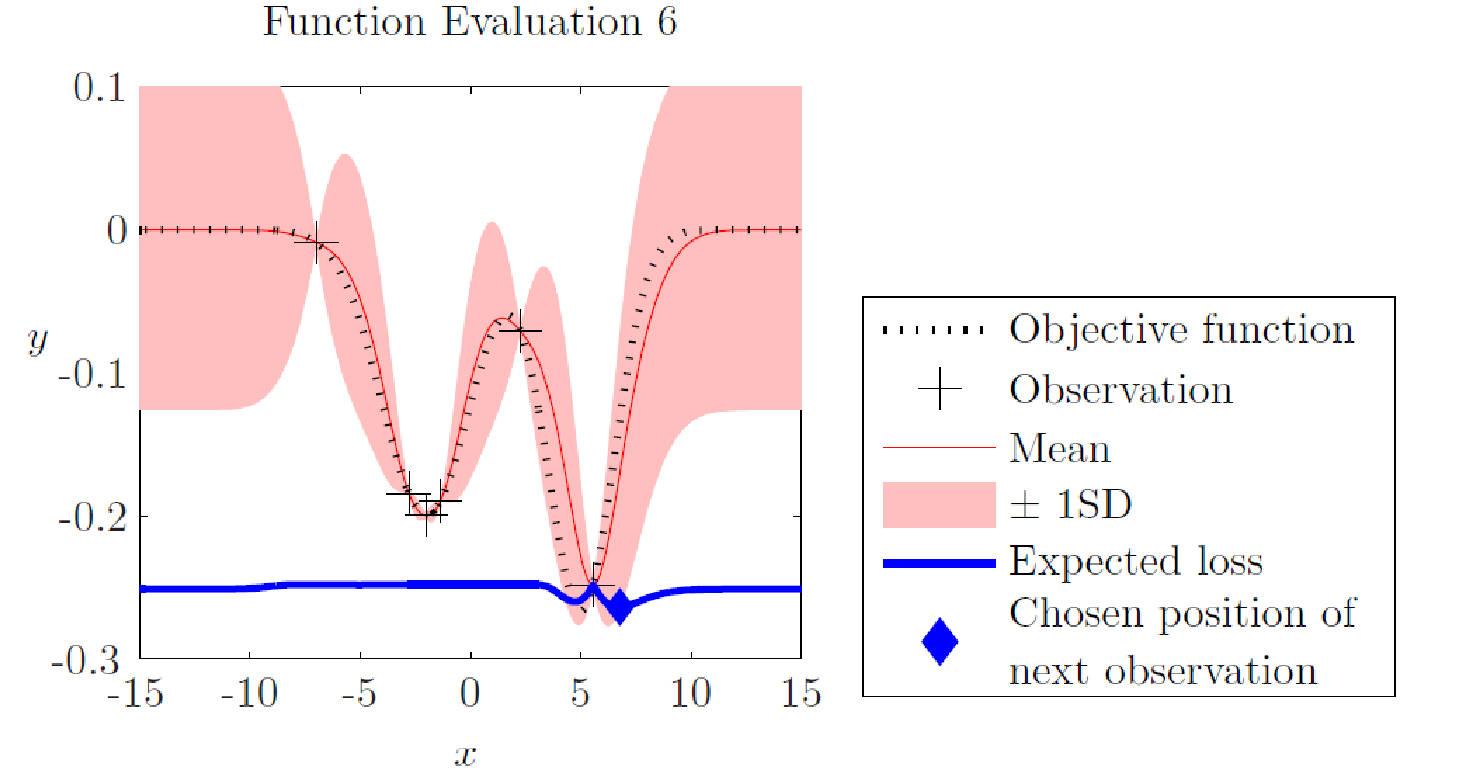
\includegraphics[width = \textwidth]{./figures/bo6.pdf}
%%%%%%%%%%%%%%%%%%%%%%%%%%%%%%%%%%%%%%%%%%%%%%%%%%
\end{frame}
%%%%%%%%%%%%%%%%%%%%%%%%%%%%%%%%%%%%%%%%%%%%%%%%%%
%%%%%%%%%%%%%%%%%%%%%%%%%%%%%%%%%%%%%%%%%%%%%%%%%%
\begin{frame}\frametitle{\red{Bayesian optimization} is efficient for expensive and multimodal functions.}
%%%%%%%%%%%%%%%%%%%%%%%%%%%%%%%%%%%%%%%%%%%%%%%%%%
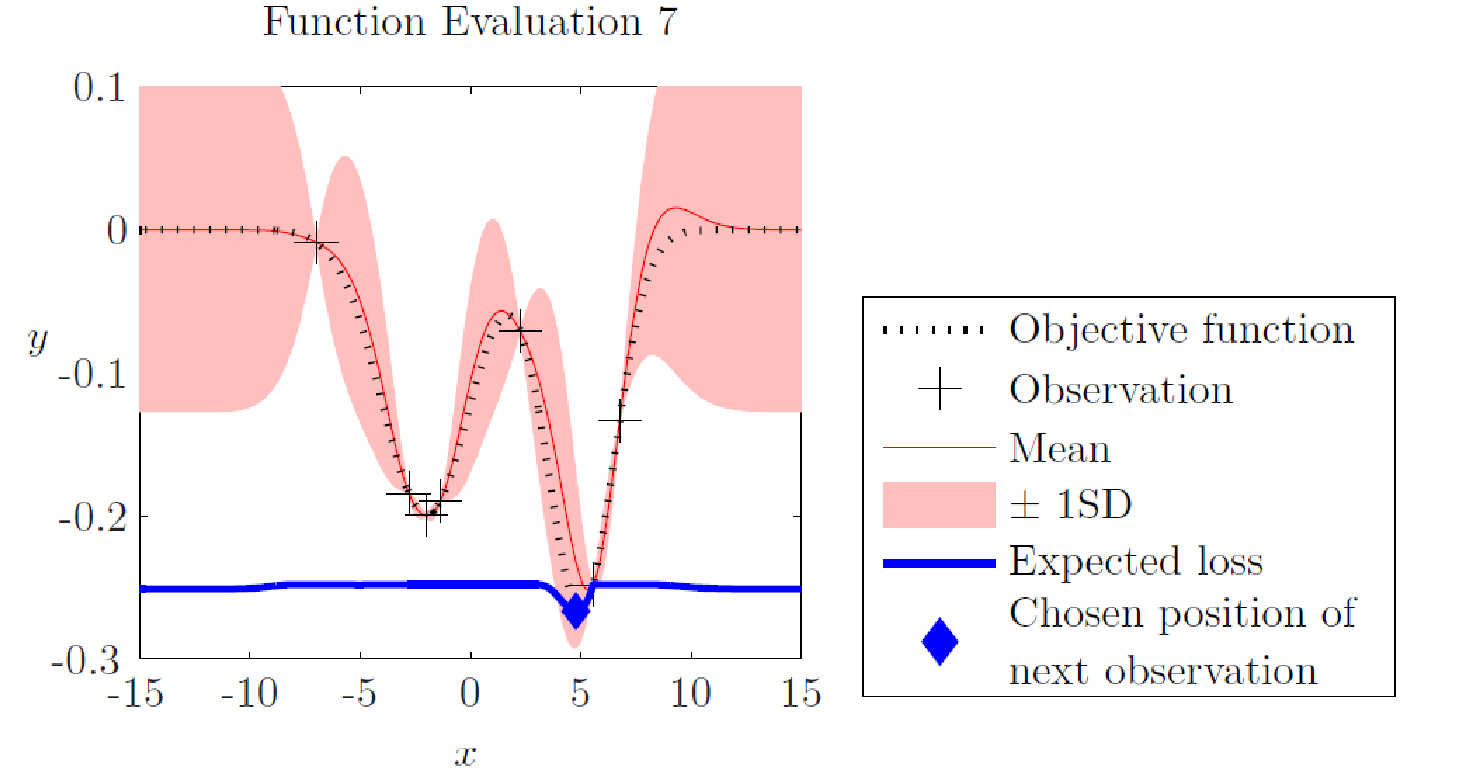
\includegraphics[width = \textwidth]{./figures/bo7.pdf}
%%%%%%%%%%%%%%%%%%%%%%%%%%%%%%%%%%%%%%%%%%%%%%%%%%
\end{frame}
%%%%%%%%%%%%%%%%%%%%%%%%%%%%%%%%%%%%%%%%%%%%%%%%%%
%%%%%%%%%%%%%%%%%%%%%%%%%%%%%%%%%%%%%%%%%%%%%%%%%%
\begin{frame}\frametitle{\red{Bayesian optimization} is efficient for expensive and multimodal functions.}
%%%%%%%%%%%%%%%%%%%%%%%%%%%%%%%%%%%%%%%%%%%%%%%%%%
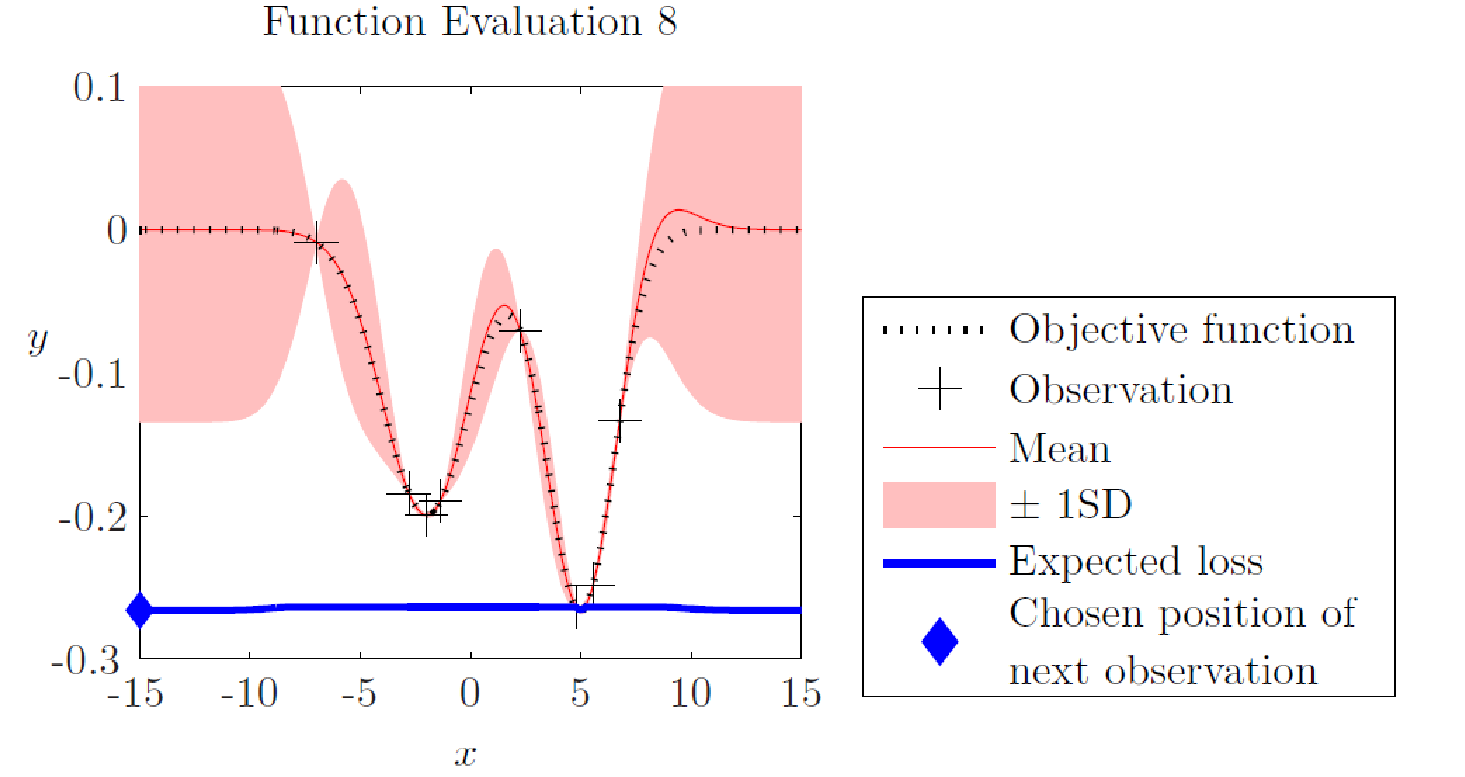
\includegraphics[width = \textwidth]{./figures/bo8.pdf}
%%%%%%%%%%%%%%%%%%%%%%%%%%%%%%%%%%%%%%%%%%%%%%%%%%
\end{frame}
%%%%%%%%%%%%%%%%%%%%%%%%%%%%%%%%%%%%%%%%%%%%%%%%%%
%%%%%%%%%%%%%%%%%%%%%%%%%%%%%%%%%%%%%%%%%%%%%%%%%%
\begin{frame}\frametitle{\red{Bayesian optimization} is efficient for expensive and multimodal functions.}
%%%%%%%%%%%%%%%%%%%%%%%%%%%%%%%%%%%%%%%%%%%%%%%%%%
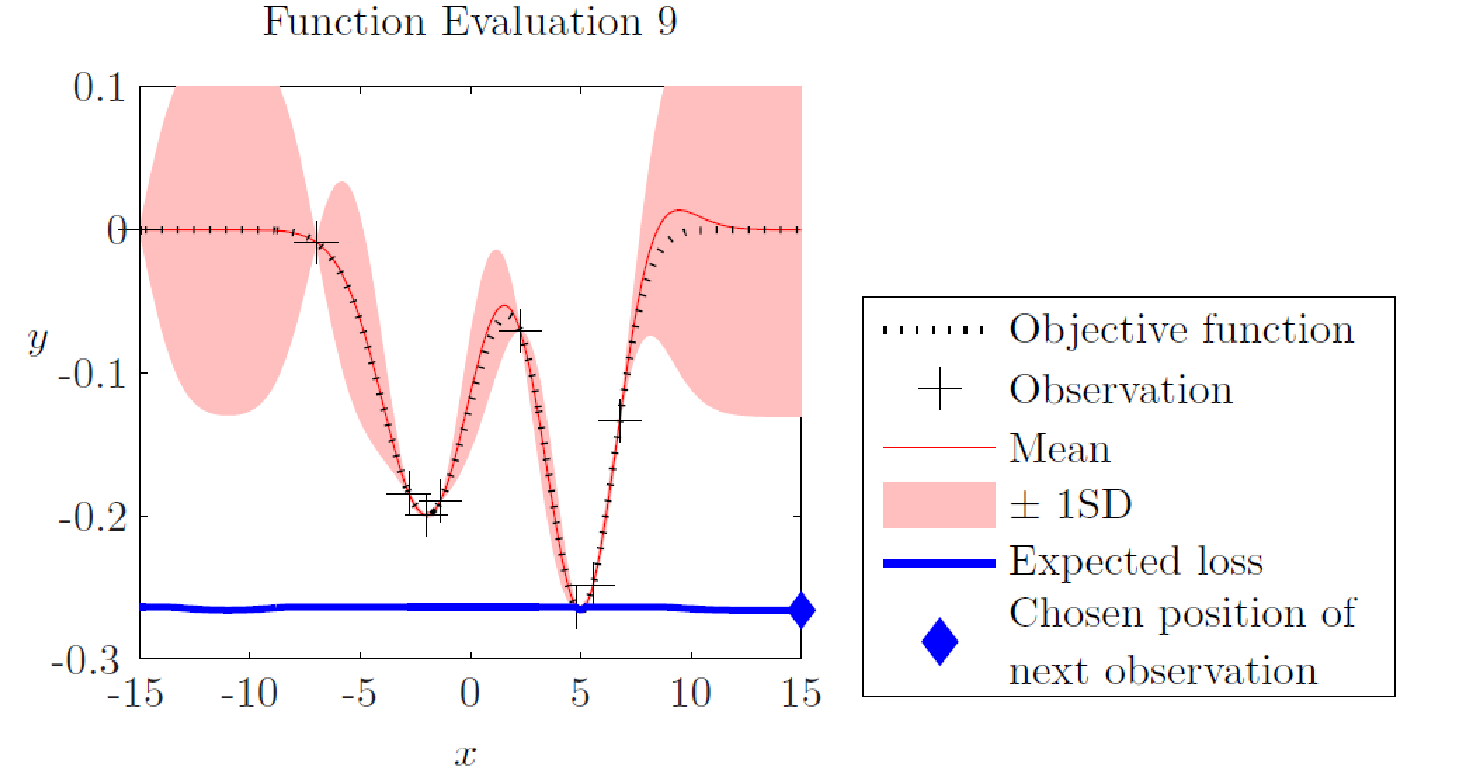
\includegraphics[width = \textwidth]{./figures/bo9.pdf}
%%%%%%%%%%%%%%%%%%%%%%%%%%%%%%%%%%%%%%%%%%%%%%%%%%
\end{frame}
%%%%%%%%%%%%%%%%%%%%%%%%%%%%%%%%%%%%%%%%%%%%%%%%%%
%%%%%%%%%%%%%%%%%%%%%%%%%%%%%%%%%%%%%%%%%%%%%%%%%%
\begin{frame}\frametitle{\red{Bayesian optimization} is efficient for expensive and multimodal functions.}
%%%%%%%%%%%%%%%%%%%%%%%%%%%%%%%%%%%%%%%%%%%%%%%%%%
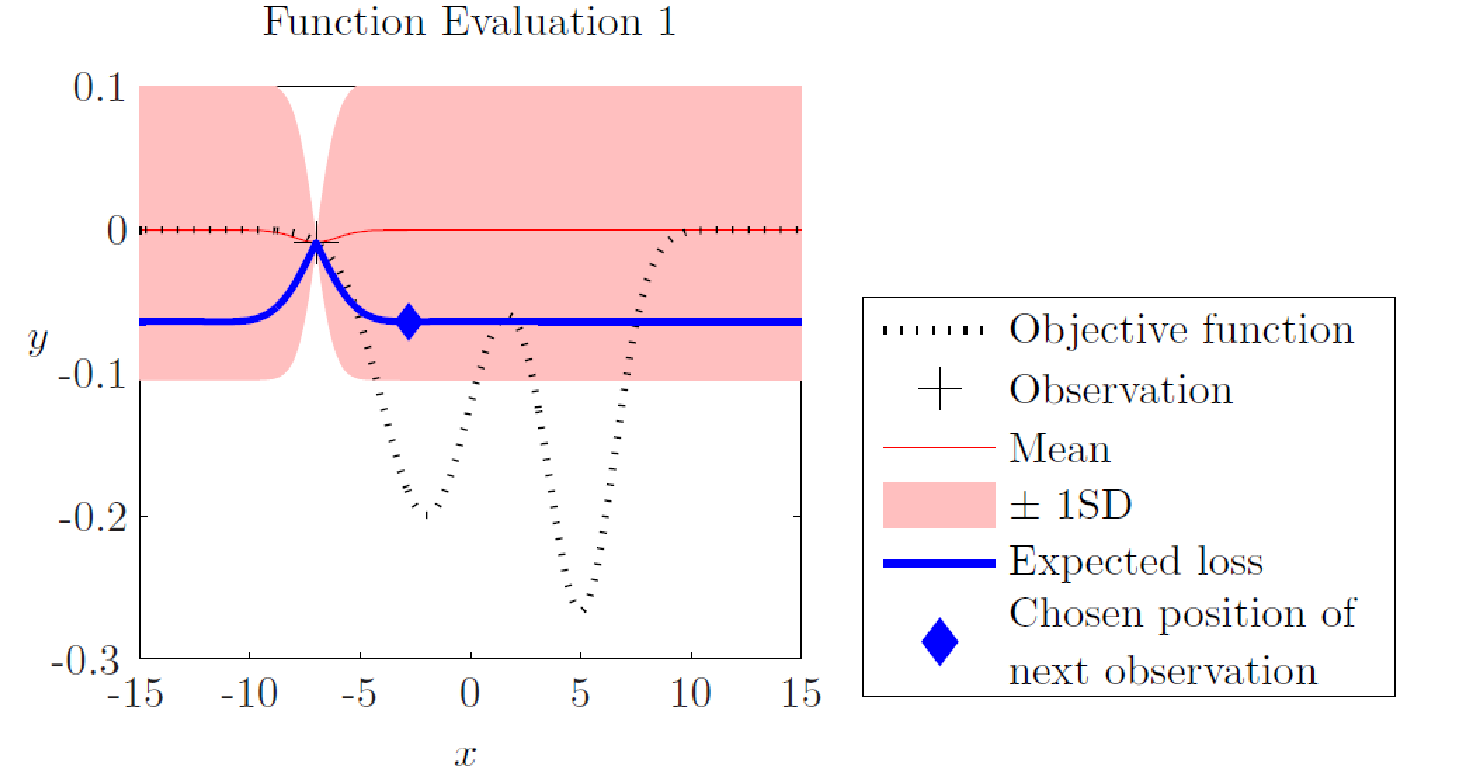
\includegraphics[width = \textwidth]{./figures/bo1.pdf}
%%%%%%%%%%%%%%%%%%%%%%%%%%%%%%%%%%%%%%%%%%%%%%%%%%
\end{frame}
%%%%%%%%%%%%%%%%%%%%%%%%%%%%%%%%%%%%%%%%%%%%%%%%%%

%%%%%%%%%%%%%%%%%%%%%%%%%%%%%%%%%%%%%%%%%%%%%%%%%%
\begin{frame}\frametitle{An increasingly important application for BayesOpt is the \orange{configuration of algorithms.}}
%%%%%%%%%%%%%%%%%%%%%%%%%%%%%%%%%%%%%%%%%%%%%%%%%%

Many algorithms have parameters that are \darkpurple{laboriously tuned by hand:} instead, why not use Bayesian Optimization?
\vfill
See, for example,
{Programming by Optimisation,}
{AutoML} and
{Spearmint.}

%%%%%%%%%%%%%%%%%%%%%%%%%%%%%%%%%%%%%%%%%%%%%%%%%%
\end{frame}
%%%%%%%%%%%%%%%%%%%%%%%%%%%%%%%%%%%%%%%%%%%%%%%%%%

%%%%%%%%%%%%%%%%%%%%%%%%%%%%%%%%%%%%%%%%%%%%%%%%%%
\begin{frame}\frametitle{Many algorithms have parameters that are \cyan{only relevant} if other inputs take \red{certain values.}}
%%%%%%%%%%%%%%%%%%%%%%%%%%%%%%%%%%%%%%%%%%%%%%%%%%
This problem arises in:
\begin{itemize}
	\item  deep neural networks \citep{HinOsiTeh06}; 
	\item  flexible computer vision architectures \citep{BerYamCox13}; 
	\item and the combined selection and hyperparameter optimization of machine learning algorithms \citep{ThoEtAl13}.
\end{itemize}
As an explicit example, we consider a deep neural network: if we set the network depth to 2 we know that the 3rd layer's hyperparameters do not have any effect (as there is no 3rd layer).
%%%%%%%%%%%%%%%%%%%%%%%%%%%%%%%%%%%%%%%%%%%%%%%%%%
\end{frame}
%%%%%%%%%%%%%%%%%%%%%%%%%%%%%%%%%%%%%%%%%%%%%%%%%%

%%%%%%%%%%%%%%%%%%%%%%%%%%%%%%%%%%%%%%%%%%%%%%%%%%
\begin{frame}\frametitle{In order to use BayesOpt, we need to define an appropriate \green{covariance (kernel) function}.
}
%%%%%%%%%%%%%%%%%%%%%%%%%%%%%%%%%%%%%%%%%%%%%%%%%%

Formally, we aim to do inference about some function $f$ with domain 
%(input space)
 $\sX$. 
\vfill
 $\sX = \prod_{i=1}^D \sX_i$ is a $D$-dimensional input space, where each individual dimension is bounded real, that is, $\sX_i = [l_i, u_i] \subset \reals$ (with lower and upper bounds $l_i$ and $u_i$, respectively).
 \vfill
We define functions 
$\delta_i\colon \sX\to \{\textnormal{true}, \textnormal{false}\}$,
 for $i \in \{1,\,\ldots,\,D\}$.
  \darkblue{$\delta_i(\vec{x})$ stipulates the relevance of the $i$th feature $x_i$ to  
%inference about 
$f(\vec{x})$.}

%%%%%%%%%%%%%%%%%%%%%%%%%%%%%%%%%%%%%%%%%%%%%%%%%%
\end{frame}
%%%%%%%%%%%%%%%%%%%%%%%%%%%%%%%%%%%%%%%%%%%%%%%%%%





%%%%%%%%%%%%%%%%%%%%%%%%%%%%%%%%%%%%%%%%%%%%%%%%%%
\begin{frame}\frametitle{Imagine a neural network with either \brown{one or two hidden layers} and \cyan{regularization parameters} for each layer, $x_1$ and $x_2$.}
%%%%%%%%%%%%%%%%%%%%%%%%%%%%%%%%%%%%%%%%%%%%%%%%%%

If $y$ represents the performance of a one layer-net with parameters $x_1$ and $x_2$, then the value $x_2$ doesn't matter, since there is no second layer to the network.
\vfill
We assume that $\delta_1(\vec{x}) = \text{true}$; that is, the regularization parameter for the first layer is always relevant.
\vfill
Recall that $\delta_2(\vec{x})$ specifies the relevance of $x_2$. 
\vfill
Hence we'll write an \darkred{input triple as $(x_1, \delta_2(\vec{x}), x_2)$.}

%%%%%%%%%%%%%%%%%%%%%%%%%%%%%%%%%%%%%%%%%%%%%%%%%%
\end{frame}
%%%%%%%%%%%%%%%%%%%%%%%%%%%%%%%%%%%%%%%%%%%%%%%%%%

%%%%%%%%%%%%%%%%%%%%%%%%%%%%%%%%%%%%%%%%%%%%%%%%%%
\begin{frame}\frametitle{A \red{kernel $k$} needs to assign a measure of \yellow{covariance between two performances.}}
%%%%%%%%%%%%%%%%%%%%%%%%%%%%%%%%%%%%%%%%%%%%%%%%%%
That is, if 
\begin{itemize}
	\item $y$ is the performance of network with parameters $(x_1, \delta_2(\vec{x}), x_2)$ and
	\item $y'$ is the performance of network with parameters $(x'_1, \delta_2(\vec{x}'), x'_2)$,
\end{itemize}
\begin{align*}
	\text{cov}(y, y') & = k\bigl((x_1, \delta_2(\vec{x}), x_2),(x'_1, \delta_2(\vec{x}'), x'_2)\bigr).
\end{align*}

%%%%%%%%%%%%%%%%%%%%%%%%%%%%%%%%%%%%%%%%%%%%%%%%%%
\end{frame}
%%%%%%%%%%%%%%%%%%%%%%%%%%%%%%%%%%%%%%%%%%%%%%%%%%


%%%%%%%%%%%%%%%%%%%%%%%%%%%%%%%%%%%%%%%%%%%%%%%%%%
\begin{frame}\frametitle{We want $k$ to be dependent on \purple{which parameters are relevant,} and the \orange{values of relevant parameters for both points.}}
%%%%%%%%%%%%%%%%%%%%%%%%%%%%%%%%%%%%%%%%%%%%%%%%%%

 % For example, consider first-layer parameters $x_1$ and $x_1'$:
%
\begin{itemize}
\item If we are comparing two points for which the same parameters are relevant, the value of any \darkpurple{unused parameters shouldn't matter,}  
\begin{align}
 & k\bigl((x_1, \textnormal{false}, x_2), (x_1', \textnormal{false}, x_2') \bigr) \nonumber\\
& = k\bigl((x_1, \textnormal{false}, x_2''), (x_1', \textnormal{false}, x_2''')\bigr),\ 
\forall x_2, x_2', x_2'', x_2''';
\end{align}
\item the covariance between a point using both parameters and a point using only one should again \darkorange{only depend on their shared parameters,}
\begin{align}
 & k\bigl((x_1, \textnormal{false}, x_2), (x_1', \textnormal{true}, x_2') \bigr) \nonumber\\
& = k\bigl((x_1, \textnormal{false}, x_2''), (x_1', \textnormal{true}, x_2''')\bigr),\ 
\forall x_2, x_2', x_2'', x_2'''.
\end{align}
\end{itemize}
%%%%%%%%%%%%%%%%%%%%%%%%%%%%%%%%%%%%%%%%%%%%%%%%%%
\end{frame}
%%%%%%%%%%%%%%%%%%%%%%%%%%%%%%%%%%%%%%%%%%%%%%%%%%




% Put another way, in the absence of any other information, this specification encodes our prior ignorance about the irrelevant (missing) parameters while still allowing us to model correlations between relevant parameters.
% %Elaborating on the first consideration:
% %

%%%%%%%%%%%%%%%%%%%%%%%%%%%%%%%%%%%%%%%%%%%%%%%%%%
\begin{frame}\frametitle{We want $k$ to be dependent on \purple{which parameters are relevant,} and the \orange{values of relevant parameters for both points.}}
%%%%%%%%%%%%%%%%%%%%%%%%%%%%%%%%%%%%%%%%%%%%%%%%%%

This implies that
\begin{align*}
k\bigl((x_1, \textnormal{false}, x_2), (x_1, \textnormal{false}, x_2') \bigr)
& = k_{\text{FF}},\ \forall x_2, x_2'\\
k\bigl((x_1, \textnormal{false}, x_2), (x_1, \textnormal{true}, x_2') \bigr)
& = k_{\text{FT}},\ \forall x_2, x_2'.
\end{align*}
\vfill
We usually additionally want 
\darkred{$$k_{\text{FF}}>k_{\text{FT}},$$}%
expressing the fact that points that have identical relevance $\delta_2({\vec{x}})$ are more similar than points that differ in relevance $\delta_2({\vec{x}})$.

%%%%%%%%%%%%%%%%%%%%%%%%%%%%%%%%%%%%%%%%%%%%%%%%%%
\end{frame}
%%%%%%%%%%%%%%%%%%%%%%%%%%%%%%%%%%%%%%%%%%%%%%%%%%

%%%%%%%%%%%%%%%%%%%%%%%%%%%%%%%%%%%%%%%%%%%%%%%%%%
\begin{frame}\frametitle{We \yellow{embed all points in Euclidean space,} $\embeddingletter\colon \sX \mapsto \reals^N$ (for our choice of $N$).}
%%%%%%%%%%%%%%%%%%%%%%%%%%%%%%%%%%%%%%%%%%%%%%%%%%

This general strategy solves the chief problem of designing kernels: ensuring that they are \darkyellow{positive semi definite (PSD).}
\vfill
That is, a \darkblue{standard Euclidean kernel} (e.g. $\exp\bigl(-(z - z')^2) $) can be used in the embedded space, which we know is PSD. 
\vfill
We consider each \darkorange{original dimension $\sX_i$ separately,} and use the embedding $\embeddingletter_i\colon \sX_i \mapsto \reals^2$ defined by
%
%To emphasize that we're in the real case, we explicitly denote the pseudometric as $d\br_i$ and the (pseudo-)isometry from $(\sX, d_i)$ to $\reals^2,d_\text{E}$ 
%as $f\br_i$. For the definitions, recall that $\delta_i(\vec{x})$ is true iff dimension $i$ is relevant given the instantiation of $i$'s ancestors in $\vec{x}$.
%
%
\begin{align*}
\embeddingletter_i\br(\vec{x}) = 
	\begin{cases}
	[0,0]^\transpose & \textrm{ if } \delta_i(\vec{x}) = \textrm{ false }\\
	\omega_i [\sin{\pi\rho_i\frac{x_i}{u_i-l_i}}, \cos{\pi\rho_i\frac{x_i}{u_i-l_i}}]^\transpose & \textrm{ otherwise.}
	\end{cases}
\end{align*}
where $\omega_i \in \mathbb{R}^+$ and $\rho_i \in [0,1]$.

%%%%%%%%%%%%%%%%%%%%%%%%%%%%%%%%%%%%%%%%%%%%%%%%%%
\end{frame}
%%%%%%%%%%%%%%%%%%%%%%%%%%%%%%%%%%%%%%%%%%%%%%%%%%


%
%%%%%%%%%%%%%%%%%%%%%%%%%%%%%%%%%%%%%%%%%%%%%%%%%%
\begin{frame}\frametitle{This embedding and a standard Euclidean kernel \cyan{satisfies our desiderata.} }
%%%%%%%%%%%%%%%%%%%%%%%%%%%%%%%%%%%%%%%%%%%%%%%%%%
\begin{figure}

	{\hspace{-1cm}% A simple figure to illustrate Mike and Frank's embedding
% Sept 2013

\newcommand{\scaleamount}{0.7}
\newcommand{\anglemin}{40}
\newcommand{\angleminplusone}{41}
\newcommand{\anglemax}{150}
\newcommand{\angleone}{70}
\newcommand{\angletwo}{120}
\newcommand{\bigradius}{3}
\newcommand{\biggerradius}{3.3}
\newcommand{\smallradius}{0.5}
\newcommand{\xtwolabelangle}{90}
\newcommand{\belowamount}{0.2cm}
\newcommand{\belowamounttwo}{0.11cm}
\newcommand{\myell}{l}
\newcommand{\embedding}{g}

%\begin{center}
%\framebox{
\begin{tikzpicture}
[trans/.style={thick,->,shorten >=2pt,shorten <=2pt,>=stealth},scale=\scaleamount, every node/.style={transform shape}]

\tikzset{state/.style={circle,draw=black, very thick,minimum size=4em}}

\def\centerarc[#1] (#2) (#3:#4:#5)% [draw options] (center) (initial angle:final angle:radius)
{ \draw[#1] (#2) ++(#3:#5) arc (#3:#4:#5);
}
	\coordinate (left) at ({\bigradius*cos(\anglemax)}, {\bigradius*sin(\anglemax)});
	\coordinate (right) at ({\bigradius*cos(\anglemin)}, {\bigradius*sin(\anglemin)});

	\coordinate (O1) at (-2, 0);
	\coordinate (O2) at (3, 1);
	
	\coordinate (left1) at ($ (left) + (O1) $);
	\coordinate (right1) at ($ (right) + (O1) $);
	\coordinate (left2) at ($ (left) + (O2) $);
	\coordinate (right2) at ($ (right) + (O2) $);
	
	% First arc
	% ==================
	
	% Draw arcs
	\centerarc[thick] (O1) (\anglemin:\anglemax:\bigradius)
	\centerarc[thick] (O1) (\anglemin:\anglemax:\smallradius)

	\draw[fill] (left1) circle (1.5pt);
	\draw (left1) node[below = \belowamount, right] {$\embedding(0, \textnormal{true}, u$)};
	
	\draw[fill] (right1) circle (1.5pt);
	\draw (right1) node[below = \belowamount] (r1below) {}
	               node[left] {$\embedding(0, \textnormal{true}, \myell)$};

	\draw[fill] (O1) circle (1.5pt);
	\draw (O1) node[below = \belowamount] (o1below) {}
	           node[left = 0.3cm] {$\embedding(0, \textnormal{false}, \cdot)$};

	\draw (left1) -- (O1) node[above] {$\rho \pi$};
	\draw (right1) -- (O1) node[midway, below] {$\omega$};
	
	
	% Second arc
	% ================================
	\centerarc[thick] (O2) (\anglemin:\anglemax:\bigradius)
	\centerarc[thick] (O2) (\anglemin:\anglemax:\smallradius)

	\draw[fill] (left2) circle (1.5pt);
	
	\draw[fill] (right2) circle (1.5pt);
	\draw (right2) node[below = \belowamount] (r2below) {};
	

	\draw[fill] (O2) circle (1.5pt);
	\draw (O2) node[below = \belowamount] (o2below) {}
                   node[right] {$\embedding(1, \textnormal{false}, \cdot)$};

	\draw[dashed] (left2) -- (O2);
	\draw[dashed] (right2) -- (O2);


	% Connect the arcs
	\draw (left1) -- (left2);
	\draw (right1) -- (right2);
	\draw[thick] (O1) -- (O2);
	
	% Draw surface
	\foreach \i in {\angleminplusone, ..., \anglemax}
	{
		\coordinate (arca) at ({\bigradius*cos(\i)}, {\bigradius*sin(\i)});
		\coordinate (arcb) at ({\bigradius*cos(\i - 1)}, {\bigradius*sin(\i - 1)});
		\coordinate (arca1) at ($ (arca) + (O1) $);
		\coordinate (arca2) at ($ (arca) + (O2) $);
		\coordinate (arcb1) at ($ (arcb) + (O1) $);
		\coordinate (arcb2) at ($ (arcb) + (O2) $);
%		\draw[green] (arca1) -- (arca2);
		\fill[fill=blue!40,fill opacity=0.8](arca1)--(arca2)--(arcb2)--(arcb1)--cycle;
	}

	\draw (right2) node[left] {$\embedding(1, \textnormal{true}, \myell)$};

	% Draw arrows showing in which direction x1 varies.
	\coordinate(x1half) at ($ (right1)!0.5!(right2) $);
	\draw (x1half) node[below = \belowamounttwo] (x1halfbelow) {$x_1$};
	\draw[trans] ($ (r1below)!0.45!(r2below) $) -- ($ (r1below)!0.3!(r2below) $);
	\draw[trans] ($ (r1below)!0.55!(r2below) $) -- ($ (r1below)!0.7!(r2below) $);

	\coordinate(x2half) at ($ (O1)!0.6!(O2) $);
	\draw (x2half) node[below = \belowamounttwo] (x2halfbelow) {$x_1$};
	\draw[trans] ($ (o1below)!0.55!(o2below) $) -- ($ (o1below)!0.4!(o2below) $);
	\draw[trans] ($ (o1below)!0.65!(o2below) $) -- ($ (o1below)!0.8!(o2below) $);

	% Draw arrows showing in which direction x2 varies.
	\coordinate (arclabel) at ($ (O1) + ({\biggerradius*cos(\xtwolabelangle)}, {\biggerradius*sin(\xtwolabelangle)}) $);
	\draw (arclabel) node {$x_2$};
	\centerarc[trans] (O1) ( \xtwolabelangle + 5  :  \xtwolabelangle + 30  :\biggerradius)
	\centerarc[trans] (O1) ( \xtwolabelangle - 5  :  \xtwolabelangle - 30  :\biggerradius)

%	\coordinate (x1) at ({\bigradius*cos(\angletwo)}, {\bigradius*sin(\angletwo)});
%	\coordinate (x2) at ({\bigradius*cos(\angleone)}, {\bigradius*sin(\angleone)});
%	\draw[fill] (x1) circle (1.5pt);
%	\draw (x1) node[above, left] {$f(x_1, \textnormal{true})$};
%	\draw[fill] (x2) circle (1.5pt);
%	\draw (x2) node[above, right] {$f(x_2, \textnormal{true})$};
\end{tikzpicture}
%}
%\end{center}
}
	%\caption{}
%  The parameter $\rho$ determines how much distance there is along the arc.
\vspace{-0.3cm}
\end{figure}
\label{fig:cylinder}

%%%%%%%%%%%%%%%%%%%%%%%%%%%%%%%%%%%%%%%%%%%%%%%%%%
\end{frame}
%%%%%%%%%%%%%%%%%%%%%%%%%%%%%%%%%%%%%%%%%%%%%%%%%%

%%%%%%%%%%%%%%%%%%%%%%%%%%%%%%%%%%%%%%%%%%%%%%%%%%
\begin{frame}\frametitle{This embedding and a standard Euclidean kernel \cyan{satisfies our desiderata.} }
%%%%%%%%%%%%%%%%%%%%%%%%%%%%%%%%%%%%%%%%%%%%%%%%%%
In our embedded space, we have the Euclidean distance,
%
\begin{align*}
d\br_i(\vec{x}, \vec{x}') & = 
||\embeddingletter_i\br(\vec{x})-\embeddingletter_i\br(\vec{x}')||_2 \nonumber\\
& = \left\{\begin{array}{ll}
0 & \textrm{ if } \delta_i(\vec{x}) = \delta_i(\vec{x}') = \textrm{false}\\
\omega_i & \textrm{ if } \delta_i(\vec{x}) \neq \delta_i(\vec{x}')\\
\omega_i \sqrt{2} \sqrt{1 - \cos(\pi\rho_i \frac{x_i-x_i'}{u_i-l_i})} & \textrm{ if } \delta_i(\vec{x}) = \delta_i(\vec{x}') = \textrm{true}. \end{array}\right.
\label{eq:distance}
\end{align*}
We can then use our favourite Euclidean covariance, e.g.
\begin{itemize}
	\item $k_i(\vec{x}, \vec{x}') = \sigma^2 \exp\bigl(-\frac{1}{2}d\br_i(\vec{x}, \vec{x}') \bigr)^2$ or
	\item $k_i(\vec{x}, \vec{x}') = \sigma^2 (1+\frac{1}{2\alpha} d\br_i(\vec{x}, \vec{x}')^2)^{-\alpha}$.
\end{itemize}
%%%%%%%%%%%%%%%%%%%%%%%%%%%%%%%%%%%%%%%%%%%%%%%%%%
\end{frame}
%%%%%%%%%%%%%%%%%%%%%%%%%%%%%%%%%%%%%%%%%%%%%%%%%%

%%%%%%%%%%%%%%%%%%%%%%%%%%%%%%%%%%%%%%%%%%%%%%%%%%
\begin{frame}\frametitle{Our embedding has \red{two parameters: $\rho$ and $\omega$.}}
%%%%%%%%%%%%%%%%%%%%%%%%%%%%%%%%%%%%%%%%%%%%%%%%%%
These two parameters weight how the relative importances of 
\begin{itemize}
	\item differing in $x_2$ while having $\delta_2({\vec{x}})=$ true and
	\item having different values for $\delta_2({\vec{x}})$.
\end{itemize}
\vfill
Explicitly, $\omega$ controls the arc radius and $\rho$ controls the arc angle.
\vfill
If $\rho$ is sufficiently small, we return to the original distance over $x_2$.
\vfill
We fit these hyperparameters using maximum likelihood or MCMC, as with any other kernel hyperparameters.
%%%%%%%%%%%%%%%%%%%%%%%%%%%%%%%%%%%%%%%%%%%%%%%%%%
\end{frame}
%%%%%%%%%%%%%%%%%%%%%%%%%%%%%%%%%%%%%%%%%%%%%%%%%%

%%%%%%%%%%%%%%%%%%%%%%%%%%%%%%%%%%%%%%%%%%%%%%%%%%
\begin{frame}\frametitle{We embed \green{each dimension separately} in $\mathbb{R}^2$, so that our final embedded space is $\mathbb{R}^{2D}$.}
%%%%%%%%%%%%%%%%%%%%%%%%%%%%%%%%%%%%%%%%%%%%%%%%%%
This gives us a kernel over the entire D-dimensional input space,
\vfill
\begin{align*}
	k(\v{x}, \v{x}') & = \prod_{i=1}^D k_i(\vec{x}, \vec{x}').
\end{align*}
\vfill
We call it the \darkpurple{arc kernel.}
%%%%%%%%%%%%%%%%%%%%%%%%%%%%%%%%%%%%%%%%%%%%%%%%%%
\end{frame}
%%%%%%%%%%%%%%%%%%%%%%%%%%%%%%%%%%%%%%%%%%%%%%%%%%

%%%%%%%%%%%%%%%%%%%%%%%%%%%%%%%%%%%%%%%%%%%%%%%%%%
\begin{frame}\frametitle{To test our kernel, we attempt to model the \green{performance of neural networks for classification.}}
%%%%%%%%%%%%%%%%%%%%%%%%%%%%%%%%%%%%%%%%%%%%%%%%%%
We consider the canonical MNIST digits dataset~\citep{lecun-1998a} where the task is to classify handwritten digits.
\vfill
We also consider the CIFAR-10 object recognition dataset~\citep{Krizhevsky-2009a}.
We pre-processed CIFAR-10 by extracting features according to the pipeline given in~\cite{coates2010analysis}.
%%%%%%%%%%%%%%%%%%%%%%%%%%%%%%%%%%%%%%%%%%%%%%%%%%
\end{frame}
%%%%%%%%%%%%%%%%%%%%%%%%%%%%%%%%%%%%%%%%%%%%%%%%%%


%%%%%%%%%%%%%%%%%%%%%%%%%%%%%%%%%%%%%%%%%%%%%%%%%%
\begin{frame}\frametitle{We tested the \purple{regression performance} of our kernel on MNIST data.}
%%%%%%%%%%%%%%%%%%%%%%%%%%%%%%%%%%%%%%%%%%%%%%%%%%
951 datapoints (performance evaluations of neural networks for different parameter settings) were generated on MNIST.  
\vfill
We then tested regression performance of different models for that data; Results are averaged over 10-fold train/test splits.
%%%%%%%%%%%%%%%%%%%%%%%%%%%%%%%%%%%%%%%%%%%%%%%%%%
\end{frame}
%%%%%%%%%%%%%%%%%%%%%%%%%%%%%%%%%%%%%%%%%%%%%%%%%%

%%%%%%%%%%%%%%%%%%%%%%%%%%%%%%%%%%%%%%%%%%%%%%%%%%
\begin{frame}\frametitle{We tested the \red{regression performance} of our kernel on MNIST data.}
%%%%%%%%%%%%%%%%%%%%%%%%%%%%%%%%%%%%%%%%%%%%%%%%%%
The `separate' models assume that performance for classifiers with different numbers of parameters (i.e. different numbers of hidden layers, different architectures) are independent. 
\vfill
\begin{table}[h!]
\caption{\small Normalized Mean Squared Error \label{tab:nn_error}}
\label{tbl:nn_nmse}
% --- Automatically generated by resultsToLatex4.m ---
% Exported at 20-Oct-2013 19:39:08
\begin{center}
\begin{tabular}{l | r r}
Method & \rotatebox{0}{ Original data   }  & \rotatebox{0}{ Log outputs }  \\ \hline
Separate Linear & $0.812 \pm 0.045$ & $0.737 \pm 0.049$ \\
Separate \gp{} & $0.546 \pm  0.038$ & $0.446 \pm 0.041$ \\
Separate \agp{} & $0.535 \pm 0.030$ & $0.440 \pm 0.031$ \\
Linear & $0.876 \pm 0.043$ & $0.834 \pm 0.047$ \\
\gp{} & $0.481 \pm 0.031$ & $0.401 \pm 0.028$ \\
\agp{} & $\mathbf{0.421 \pm  0.033}$ & $\mathbf{0.335 \pm 0.028}$
\end{tabular}
\end{center}
% End automatically generated LaTeX

%% --- Automatically generated by resultsToLatex4.m ---
% Exported at 20-Oct-2013 19:39:08
\begin{center}
{\small
\begin{tabular}{l | r r r r r r}
Method & Separate Linear & Separate \gp{} & Separate \agp{} & Linear & \gp{} &\agp{} \\ \hline
Original data & $0.812 \pm 0.045$ & $0.546 \pm 0.038$ & $0.535 \pm 0.030$ & $0.876 \pm 0.043$ & $0.481 \pm 0.031$ & $\mathbf{0.421 \pm 0.033}$ \\
Log outputs   & $0.737 \pm 0.049$ & $0.446 \pm 0.041$ & $0.440 \pm 0.031$ & $0.834 \pm 0.047$ & $0.401 \pm 0.028$ & $\mathbf{0.335 \pm 0.028}$ \\
\end{tabular}
}
\end{center}
% End automatically generated LaTeX

%\caption{Regression errors for a GP with the arc kernel compared to baselines.}
\vspace{-0.3cm}
\end{table}
%%%%%%%%%%%%%%%%%%%%%%%%%%%%%%%%%%%%%%%%%%%%%%%%%%
\end{frame}
%%%%%%%%%%%%%%%%%%%%%%%%%%%%%%%%%%%%%%%%%%%%%%%%%%

%%%%%%%%%%%%%%%%%%%%%%%%%%%%%%%%%%%%%%%%%%%%%%%%%%
\begin{frame}\frametitle{We next evaluated using the arc kernel to perform \orange{Bayesian optimisation.}}
%%%%%%%%%%%%%%%%%%%%%%%%%%%%%%%%%%%%%%%%%%%%%%%%%%
We test the ability of Bayesian optimization to tune the hyperparameters of each layer of a \darkblue{deep neural network.}
\vfill
We allow the neural networks for these problems to use up to $5$ hidden layers (or no hidden layer).
\vfill
We optimize over learning rates, L2 weight constraints, dropout rates~\cite{hinton2012improving}, and the number of hidden units per layer leading to a total of up to $23$ hyperparameters and $6$ architectures.
\vfill
Our baseline is \darkpurple{BayesOpt with a GP that assumes random values for irrelevant parameters.}
%%%%%%%%%%%%%%%%%%%%%%%%%%%%%%%%%%%%%%%%%%%%%%%%%%
\end{frame}
%%%%%%%%%%%%%%%%%%%%%%%%%%%%%%%%%%%%%%%%%%%%%%%%%%

%%%%%%%%%%%%%%%%%%%%%%%%%%%%%%%%%%%%%%%%%%%%%%%%%%
\begin{frame}\frametitle{We have results on the \blue{MNIST problem.}}
%%%%%%%%%%%%%%%%%%%%%%%%%%%%%%%%%%%%%%%%%%%%%%%%%%
\begin{figure}[t!]
	\centering
		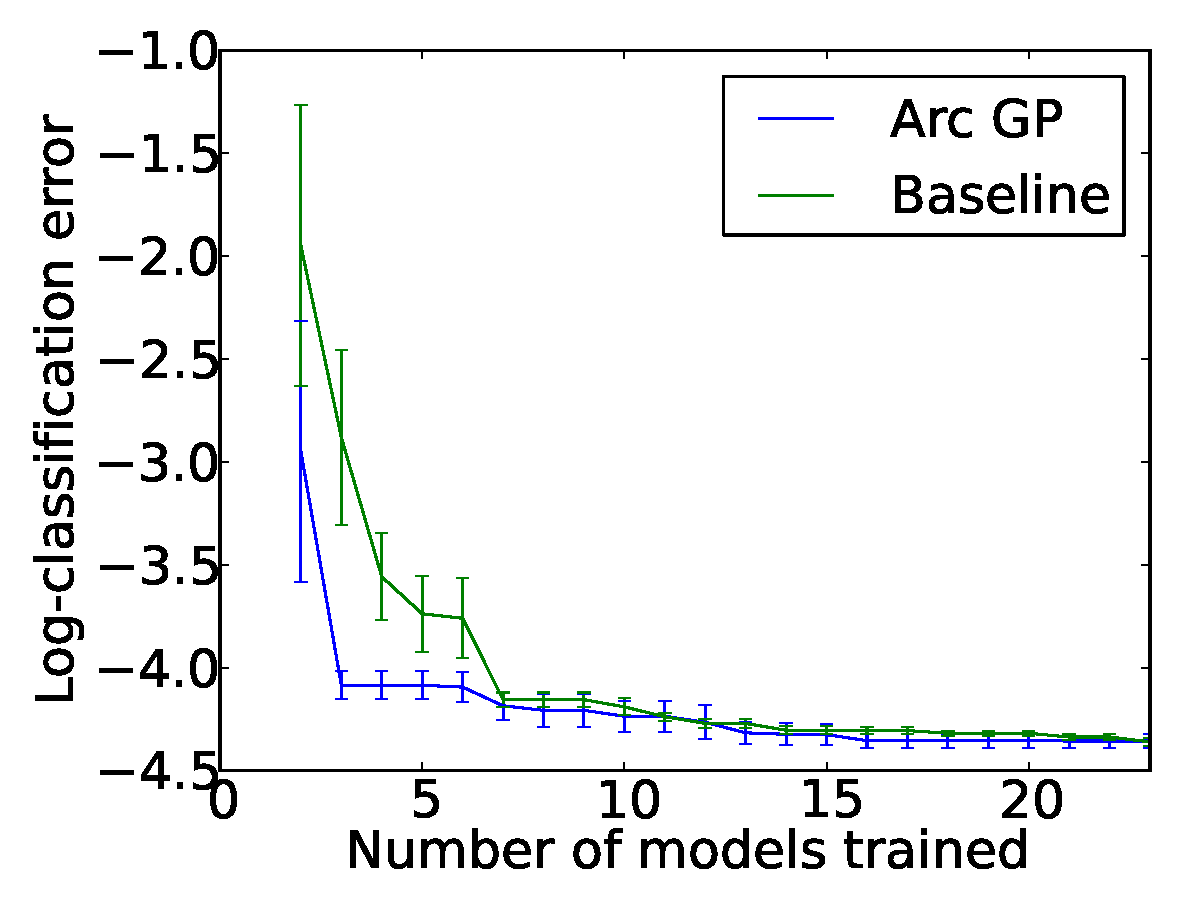
\includegraphics[width=0.9\columnwidth]{figures/mnist}
		\label{fig:mnist}
\end{figure}


%%%%%%%%%%%%%%%%%%%%%%%%%%%%%%%%%%%%%%%%%%%%%%%%%%
\end{frame}
%%%%%%%%%%%%%%%%%%%%%%%%%%%%%%%%%%%%%%%%%%%%%%%%%%
%%%%%%%%%%%%%%%%%%%%%%%%%%%%%%%%%%%%%%%%%%%%%%%%%%
\begin{frame}\frametitle{We have results on the \purple{CIFAR-10 problem.}}
%%%%%%%%%%%%%%%%%%%%%%%%%%%%%%%%%%%%%%%%%%%%%%%%%%


\begin{figure}[t!]
	\centering
		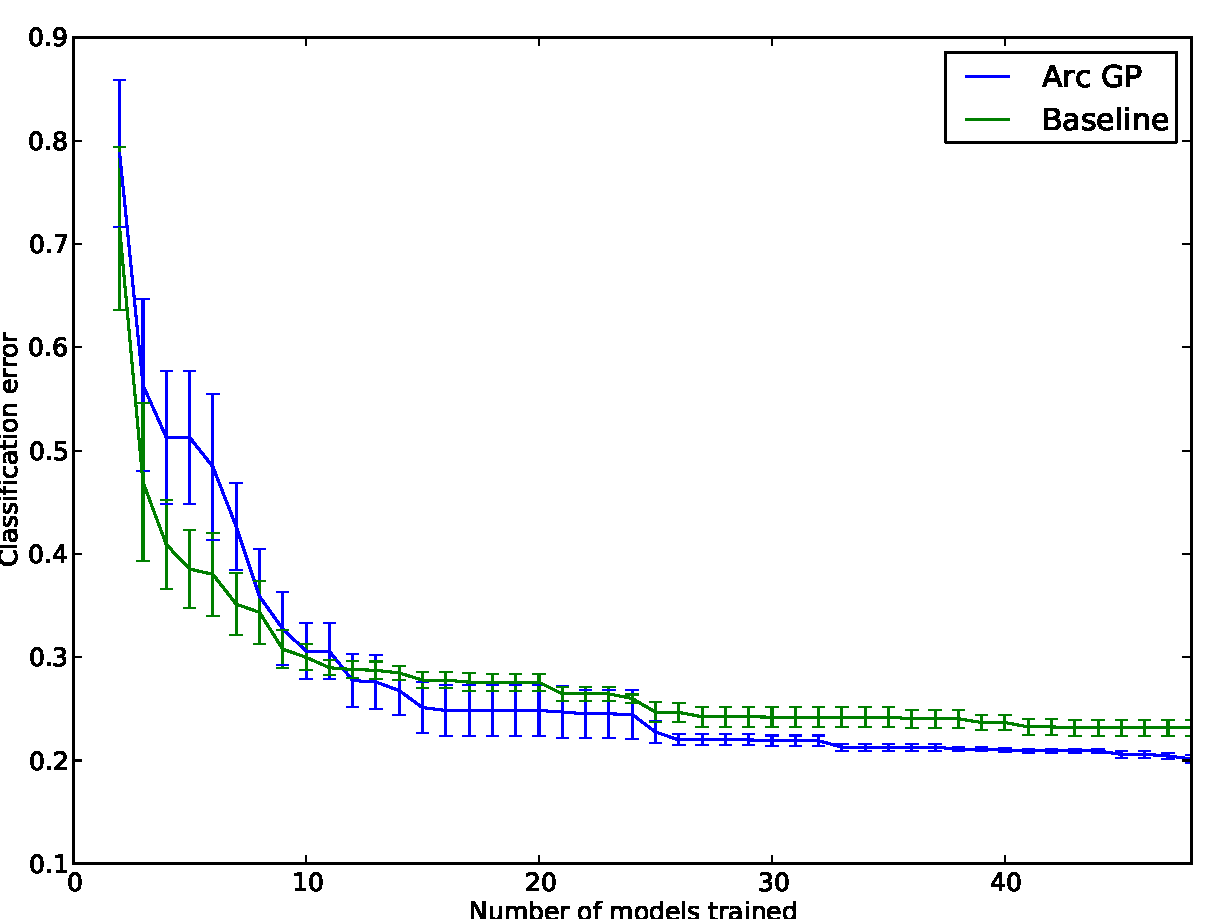
\includegraphics[width=0.9\columnwidth]{figures/cifar10}
		\label{fig:cifar10}
\end{figure}


%%%%%%%%%%%%%%%%%%%%%%%%%%%%%%%%%%%%%%%%%%%%%%%%%%
\end{frame}
%%%%%%%%%%%%%%%%%%%%%%%%%%%%%%%%%%%%%%%%%%%%%%%%%%
%%%%%%%%%%%%%%%%%%%%%%%%%%%%%%%%%%%%%%%%%%%%%%%%%%
\begin{frame}\frametitle{We search over \cyan{deeper architectures} for the CIFAR-10 experiment.}
%%%%%%%%%%%%%%%%%%%%%%%%%%%%%%%%%%%%%%%%%%%%%%%%%%


\begin{figure}[t!]
	\centering
		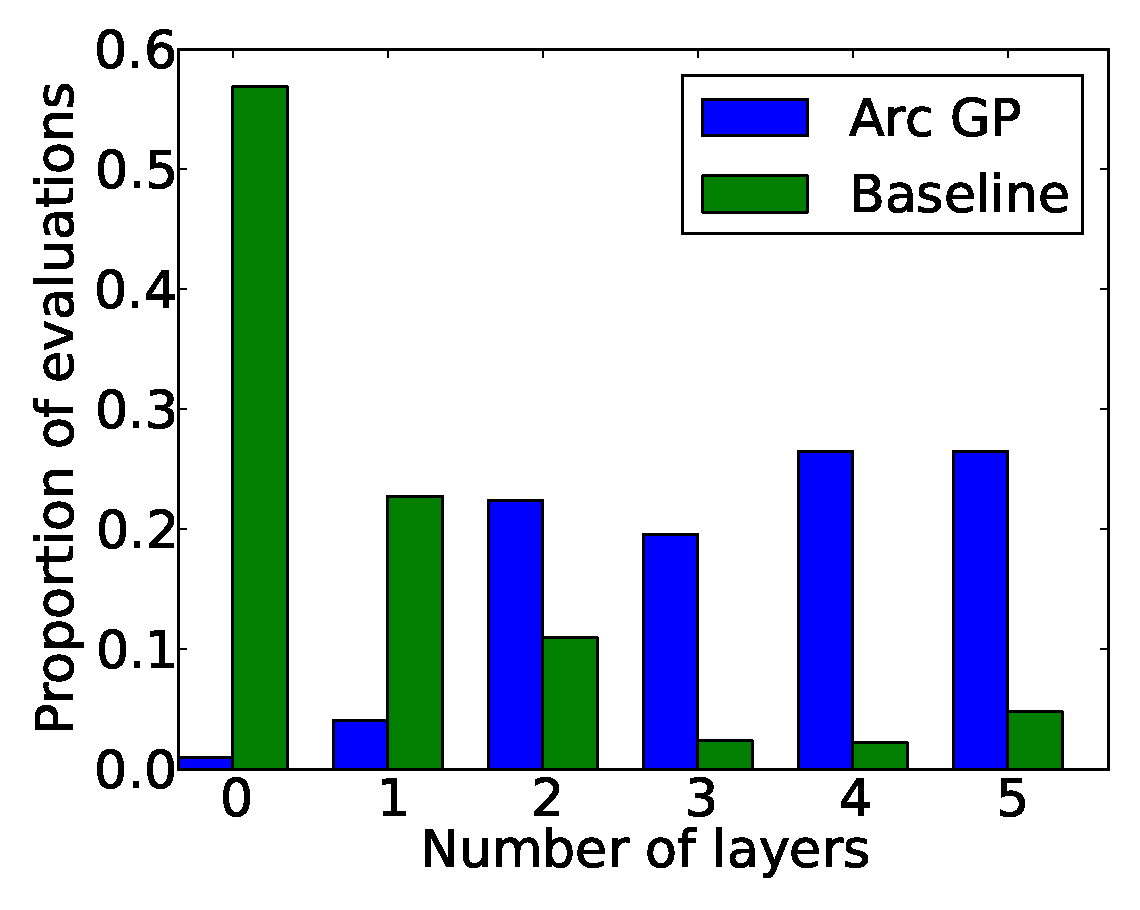
\includegraphics[width=0.8\columnwidth]{figures/fevals_per_layer}
		\caption{Architectures searched}
		\label{fig:proparchs}
\end{figure}

%%%%%%%%%%%%%%%%%%%%%%%%%%%%%%%%%%%%%%%%%%%%%%%%%%
\end{frame}
%%%%%%%%%%%%%%%%%%%%%%%%%%%%%%%%%%%%%%%%%%%%%%%%%%

%%%%%%%%%%%%%%%%%%%%%%%%%%%%%%%%%%%%%%%%%%%%%%%%%%
\begin{frame}\frametitle{The \red{arc kernel} finds better solutions faster.}
%%%%%%%%%%%%%%%%%%%%%%%%%%%%%%%%%%%%%%%%%%%%%%%%%%
Allowing information to be shared across architectures improves the efficiency of Bayesian optimization and removes the need to manually search for good architectures.
\vfill
The resulting models perform favourably compared to established benchmarks by domain experts.
%%%%%%%%%%%%%%%%%%%%%%%%%%%%%%%%%%%%%%%%%%%%%%%%%%
\end{frame}
%%%%%%%%%%%%%%%%%%%%%%%%%%%%%%%%%%%%%%%%%%%%%%%%%%


% Kevin, would it be possible to run on a dataset where we know larger
% (deeper) models will overfit?  I guess the sentiment these days in the deep
% learning world is that you should take the largest model you can and apply
% sufficient dropout.  Of course, the naive baseline will prefer the
% larger/more parameterized models because the uncertainty there is greatest
% (right?).  So it's basically annoying coincidence that the baseline does
% well here.

% 10+ layers are still difficult to train right?  Maybe this will be
% reflected in the experiments!


% I'm going to start getting some plots together today, but the baseline
% does look strong. I think on this data 3, 4, and 5 layer nets all have
% settings that do well, and the baseline (which defaults values to 0)
% heavily favours 5 layer models. Basically, I think it's just doing
% regular search on the space of 5 layer nets.

% There is possibly an argument to be made that more layers = more
% computation, so I'll get some cumulative model training time plots as
% well to see if that helps us.

% I modified the code to use up to 10 layers (actually it can go up to
% an arbitrary number, but I'm searching up to 10). I removed dropout
% and reduced the number of training updates to 20K instead of 100K
% (dropout makes training much slower). I'm doing a trial run to see how
% this goes, but it actually seems quite fast. If it's looking promising
% I'll upload this version to the repo for SMAC/TPE comparisons.

% MNIST is easy, but a good sanity check. Cifar is a bit harder, but it
% still had quite a bit of multimodality. Removing dropout should make
% it more difficult to regularize super deep models though, so hopefully
% this bears some fruit.

% Preliminary findings are showing that the same story holds, even with
% 10 layers! wtf!

% I guess the conclusion here is that once you hit a certain
% architecture size with these problems then the number of layers
% becomes irrelevant. Frank, I wonder if your own search supports this
% conclusion?

% 	FH: Interesting. I actually don't know since we haven't studied very deep
% 	networks before - James Bergstra's net had a max. of 3 layers, and 3 tended
% 	to do better than 2.

% If it does then David and I think we should try to spin this into more
% of an analysis of this effect. We can show the results of the arc
% kernel + baseline along with some measurements of how they differ in
% their behaviour, and then we can do some analysis of the findings
% (like how similar different architectures are and such).

% Is this reasonable?

% 	It is a surprising finding, and surprising findings tend to be interesting,
% 	particularly if they help us understand a process better.
% 	I would be extremely surprised if this finding still holds for smaller
% 	datasets.
% 	Say we fit a 10-layer network without dropout using only 1000 data points -
% 	there's gotta be overfitting!

% 	Which actually raises a question: have you looked at test performance, or
% 	only at validation performance? Validation performance will improve since
% 	that's the objective function for Bayesian optimization. The obvious fix
% 	would be cross-validation, which would penalize the deeper nets for their
% 	overfitting. But cross-validation takes longer to optimize, so I doubt we'd
% 	have this ready until Friday. If I had one shot at this experiment I'd take
% 	a small dataset, a network with up to 10 layers, and 5-fold CV.

% 	If the very deep nets really don't overfit I think that would be so
% 	surprising it's worth a paper. In the much more likely case that they do
% 	overfit with small datasets (and assuming we're not already seeing
% 	overfitting for the full dataset) I think the story could be that the
% 	dataset can be surprisingly small without incurring overfitting, and that
% 	we found that out as a side effect of being able to search over
% 	architectures effectively.

% Also with regards to the difference between the baseline here and with
% the workshop, for the workshop I didn't set the remaining variables to
% a default value, I just kept them the way spearmint suggested them. I
% think your baselines for your workshop paper would have done the same
% since it used the default spearmint.

% Thinking about it in hindsight, the effect this would have is that
% there would be a great deal of uncertainty, even with smaller
% architectures. For example, consider two 0-layer architectures with
% identical 0-layer parameters but random irrelevant parameters. These
% would return the same result, but would be considered as different
% inputs to the GP, so there would be a lot of artificial uncertainty
% around this.

% Contrast that with default value approach, there two 0-layer
% architectures with identical 0-layer parameters would always represent
% the same input to a GP, drastically reducing the uncertainty. The most
% uncertainty would be found when more parameters are allowed to vary,
% as would be found in a large architecture.

% 	This is quite frustrating!  I wonder if there is a way to penalize the
% 	larger networks.  E.g. we would like to find the smallest network that does
% 	well on a given problem.  That's perhaps opening a whole new can of worms.

% 	I think analysis is certainly interesting.  Even the observation that using
% 	a reasonable default value vs. a random value which we were doing before is
% 	useful empirically and interesting!

% 	Aha! That's an interesting finding, and certainly a point we should hit
% 	hard in the empirical results:
% 	- the regular Spearmint was stupid about irrelevant parameters and thus
% 	performed poorly,
% 	- one surprisingly strong fix is to simply impute default values for
% 	irrelevant parameters, and
% 	- a more principled fix is the new kernel.

% 	The story would be even better if we could show that imputing default
% 	values has other annoying side-effects (e.g., spending all its time in the
% 	deepest network, even if that overfits like crazy for small datasets).

% 	@Kevin: We should have anything that you'd like us to run TPE/SMAC on by
% 	German Thursday morning (i.e., when you go to bed Wednesday). That'll give
% 	us time to set up the experiments + 24h of runtime (which many of the
% 	scenarios need)!

% 	We can then discuss the surprising result that 5-layer nets do just as
% 	well if not better than smaller nets. To test this further we then do
% 	an experiment with 10 layer nets and no droupout so that overfitting
% 	becomes a serious problem. Surprisingly, the best nets still tend to
% 	have lots of layers, they just tend to be skinny (I think this is what
% 	the data says but will look closer).

% 	As dicussed with Kevin, here's the storyline as it could potentially flow:
% 	- old Spearmint baseline from the workshop vs. arc kernel from workshop vs
% 	new arc kernel, on MNIST & CIFAR-10
% 	- comparison of those to SMAC & TPE (crossing my fingers that we'll have
% 	results tomorrow)

% 	- also compare to the new baseline (default imputation) -> surprising
% 	finding that it performs best
% 	- explain that finding: it prefers deepest (5-layer) nets, which perform
% 	best
% 	- thus move to 10 layers without dropout for the next experiment & cross
% 	our fingers that deepest is not best anymore and that thus the new baseline
% 	is not the best anymore...

% 	Note that for the text this will mean that we'll describe both the simple
% 	arc kernel from the workshop and the newer one. The experiments seem to
% 	also show the newer one to be better. That will also fill space in a
% 	meaningful way, explaining two contributions.
% 	Do we actually have regression results for both types of arc kernel, to
% 	mirror the experiments in the regression setting?

% 		Unfortunately the data wasn't coming back in our favour. The naive
% 		baseline performed too well against our proposal, even in the
% 		ridiculous scenario of 10 layers. My guess is that because the
% 		baseline favoured deeper nets, it effectively became a matter of just
% 		applying spearmint to an 8/9/10 layer architecture. This would
% 		certainly perform better than doing a thorough exploration of the
% 		whole space as long as the hypothesis of "depth doesn't hurt" holds.

% 		So for now I think I'm going to have to call this. It was a good push
% 		and yielded a lot of interesting results, but we just wouldn't be able
% 		to wrap it up into a coherent story in time.

% 		When I get back to research I'm going to run out a search over n-layer
% 		fixed architectures to see how far each of them can be pushed
% 		independently. This will give us a baseline over which to evaluate any
% 		future methods.

% 		Some possibilities to consider:
% 		1) Training greedily layer by layer, using the previous search to
% 		bootstrap a new one, in order to find the smallest possible
% 		architecture that does well.
% 		2) Trying EI/s instead of EI as the acquisition function, to bias them
% 		toward smaller models (not necessarily shallower, but thinner as
% 		well).
% 		3) Other kernels: for example we can infer the default value rather
% 		than just setting it, then the box kernel is an extension of this, and
% 		finally whatever Roman's cooking up.
% 		4) Some independent tests for the categorical kernel.
% 		5) Other problems where choosing the wrong conditional variables
% 		actually matter.
% 		6) Convolutional nets may not exhibit the behaviour we've seen here,
% 		and so the story may change when going that route.

% 		There is also another thread of research emerging from this with
% 		respect to analyzing deep nets. I've already got an undergrad who's
% 		working on this so it's a bit of a coincidence that this happened, but
% 		the result that we might be able to find good settings for really deep
% 		architectures is interesting. It certainly merits further
% 		investigation.

% 		Any other thoughts?

% 		Thank you all for your hard work!

% \section{Missing Data}

% Besides being useful for sharing information between architectures with differing numbers of parameters,
% conditional parameter spaces are a natural fit for the problem of missing data, when the data is not missing at random. [cite]

% As an example, consider the problem of estimating creditworthiness from loan applications.
% In this setting, credit score is a strong indicator of creditworthness.
% However, if a loan applicant doesn't report a credit rating, or has no credit rating, this is very informative about their creditworthiness.

% The arc kernel lets us flexibly model the significance the absense of any piece of data, without requiring expensive imputation.

% %%%%%%%%%%%%%%%%%%%%%%%%%%%%%%%%%%%%%%%%%%%%%%%%%%
% \begin{frame}\frametitle{We can also use our kernel to handle data \red{missing not-at-random.}}
% %%%%%%%%%%%%%%%%%%%%%%%%%%%%%%%%%%%%%%%%%%%%%%%%%%

% \begin{figure}
%   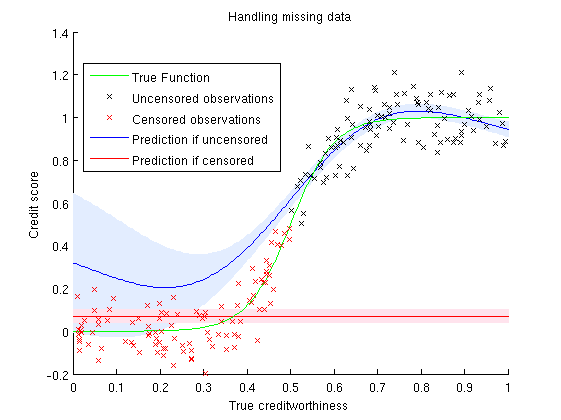
\includegraphics[width=0.8\columnwidth]{figures/missing_data_demo}
% \end{figure}
% % Demonstrating how the arc kernel can be used for regression under data missing-not-at-random.
% The arc kernel learns that no credit score indicates low creditworthiness.
% %%%%%%%%%%%%%%%%%%%%%%%%%%%%%%%%%%%%%%%%%%%%%%%%%%
% \end{frame}
% %%%%%%%%%%%%%%%%%%%%%%%%%%%%%%%%%%%%%%%%%%%%%%%%%%


\bibliographystyle{plainnat}

\newsavebox\mytempbib
\savebox\mytempbib{\parbox{\textwidth}{\bibliography{hierarchicalkernel}}}

\end{document}

